\documentclass[output=paper,chinesefont,colorlinks,citecolor=brown]{langscibook} 
\ChapterDOI{10.5281/zenodo.7353599}
\title{Introducing the Negative Existential Cycle} 
\author{Ljuba Veselinova\affiliation{University of Stockholm}  and Arja Hamari\affiliation{University of Helsinki;University of Turku}}
\abstract{\noabstract}

\IfFileExists{../localcommands.tex}{
   % add all extra packages you need to load to this file

\usepackage{tabularx,multicol}
\usepackage{url}
\urlstyle{same}

\usepackage{listings}
\lstset{basicstyle=\ttfamily,tabsize=2,breaklines=true}

\usepackage{langsci-optional}
\usepackage{langsci-lgr}
\usepackage{langsci-gb4e}

%from elena-----------------------------------
\usepackage{pgfplots,pgfplotstable}
\definecolor{lsDOIGray}{cmyk}{0,0,0,0.45}
\usepackage{xassoccnt}
\newcounter{realpage}
\DeclareAssociatedCounters{page}{realpage}
\AtBeginDocument{%
  \stepcounter{realpage}
}
\usepackage{enumitem}
\usepackage[]{longtable}
\usepackage{comment}

%from Nina K.---------------------------------
\usepackage{csquotes}
%\usepackage{expex}
\pgfplotsset{compat=1.16} % Why?
% \usepackage{xeCJK}
% \setCJKmainfont{HanaMinA}
\usepackage{rotating}
\usepackage{colortbl}
\usepackage{multirow}
\usepackage{dirtree}

%from Niina-----------------------------------
\usepackage{verbatim}
\usetikzlibrary{intersections, backgrounds, shapes, angles, quotes,
decorations.pathmorphing, arrows.meta, decorations.text, tikzmark}
% positioning and calc are loaded by document class
	\tikzset{snake it/.style={decorate, decoration=snake}}
\usepackage{tikz-qtree}

% figures side-by-side with body text:
\usepackage{wrapfig}
\usepackage{subcaption}

%\usepackage{enumerate}
%\usepackage[nonumberlist]{glossaries}


\usepackage[linguistics,edges]{forest}
\usetikzlibrary{positioning}
\usepackage{soul}
\usepackage{langsci-bidi}
\usepackage{langsci-branding}

   \newcommand*{\orcid}{}

%-------------------from Elena------------------------------------------------------------

\newcommand{\appref}[1]{Appendix \ref{#1}}
\newcommand{\fnref}[1]{Footnote \ref{#1}} 

\newenvironment{langscibars}{\begin{axis}[ybar,xtick=data, xticklabels from table={\mydata}{pos}, 
        width  = \textwidth,
	height = .3\textheight,
    	nodes near coords, 
	xtick=data,
	x tick label style={},  
	ymin=0,
	cycle list name=langscicolors
        ]}{\end{axis}}
        
\newcommand{\langscibar}[1]{\addplot+ table [x=i, y=#1] {\mydata};\addlegendentry{#1};}

\newcommand{\langscidata}[1]{\pgfplotstableread{#1}\mydata;}


% for annotations above example lines:
\newcommand{\overnote}[1]{\makebox[0pt][l]{\raisebox{\baselineskip}{\upshape
#1}}}
\newcommand{\moreovernote}[1]{\makebox[0pt][l]{\raisebox{2\baselineskip}{\upshape #1}}}

%--------------------from Niina----------------------------------------------------------

% \makeatletter
% \def\blx@maxline{77}
% \makeatother

% An Arabic font added to `fonts' folder, it's free and open-source
% When run on Windows, LaTeX may need the complete file name of the font:
% Amiri-Regular.ttf
% \newfontfamily\arabfont{Amiri}
% \newcommand\textarab[1]{{\arabfont #1}}%%% \textarab{...}




\newcommand{\todoref}[1]{\todo[color=green!40]{#1}}%%% 
\newcommand{\todofix}[1]{\todo[color=blue!40]{#1}}%%% 

\DeclareBibliographyCategory{sources}% filter some references
\DeclareBibliographyCategory{online}

% draw a thick bar of desired length (used for visual presentation in a
% tabular)
\newcommand{\cocabar}[1]{\color{gray}\rule[1pt]{{#1}mm}{1ex}}

% to preserve original formatting in an appendix:
\newenvironment{unindented}[0]{\setlength{\parindent}{0pt}\setlength{\parskip}{1ex
plus 0.5ex minus 0.2ex}}{}
% for annotations above example lines:
%\newcommand{\overnote}[1]{\makebox[0pt][l]{\raisebox{\baselineskip}{\upshape
%#1}}}
%\newcommand{\moreovernote}[1]{\makebox[0pt][l]{\raisebox{2\baselineskip}{\upshape #1}}}

\definecolor{blech}{rgb}{.78,.78.,.62}
\definecolor{ochre}{cmyk}{0, .42, .83, .20}
\newcommand{\exem}[1]{\textit{\textbf{#1}}}
\newcommand{\glem}[1]{\MakeUppercase{\scriptsize{\textbf{#1}}}} 
\newcommand{\denote}[1]{\mbox{$[\![\mbox{#1}]\!]$}}

\newcommand{\stacktwo}[2]{\makebox[0pt][l]{\hspace{.5pt}#1}#2}

%------------------from Nina K.-------------------------------

\newcommand{\citealtv}[1]{\citealt{#1} [this volume]}


% \renewcommand{\textdblhyphen}{⹀}


% \newcommand{\ꜥ}{\textsf{ꜥ}}
\newcommand{\ꜥ}{ʿ}
\newcommand{\ꜣ}{\kern-.25pt\texttt{ꜣ}\kern-.6pt}


\makeatletter
\let\thetitle\@title
\let\theauthor\@author
\makeatother


\newcommand{\togglepaper}[1][0]{
   \bibliography{../localbibliography}
   \papernote{\scriptsize\normalfont
     \theauthor.
     \titleTemp.
     To appear in:
     Change Volume Editor \& in localcommands.tex
     Change volume title in localcommands.tex
     Berlin: Language Science Press. [preliminary page numbering]
   }
   \pagenumbering{roman}
   \setcounter{chapter}{#1}
   \addtocounter{chapter}{-1}
}


\newfontfamily\arabicfont[Script=Arabic,ItalicFont=*,Scale=1.4]{ScheherazadeRegOT_Jazm.ttf}
% \newcommand{\arabscript}[1]{\RL{\Parsifont #1}}
\newcommand{\textarab}[1]{{\arabicfont #1}}



\DeclareCiteCommand{\textCitetv}
  {\usebibmacro{prenote}}
  {\ifciteindex
     {\indexnames{labelname}}
     {}%
   \printtext[bibhyperref]{\printnames{labelname}\addspace\bibopenparen\printfield{year}}}
  {\multicitedelim}
  {\printtext[bibhyperref]{\usebibmacro{postnote}\addspace[this volume]\bibcloseparen}}


\colorlet{karlgrencol}{pink}
\colorlet{normancol}{green}
\colorlet{pancol}{blue}
\colorlet{ohtacol}{gray}
\colorlet{peyraubecol}{orange}
\colorlet{peyraubecolmod}{yellow}
\colorlet{wangcol}{red}

\DeclareNewSectionCommand
  [
    counterwithin = appendixsubsection,
    beforeskip=-10pt,
    afterskip=1sp,
    indent = 0pt,
    font = \usekomafont{subsubsection},
    level = 3,
    tocindent = 7.0em,
    toclevel = 3,
    tocnumwidth = 4.1em,
    tocstyle = section,
    style = section
  ]
  {appendixsubsubsection}

   %% hyphenation points for line breaks
%% Normally, automatic hyphenation in LaTeX is very good
%% If a word is mis-hyphenated, add it to this file
%%
%% add information to TeX file before \begin{document} with:
%% %% hyphenation points for line breaks
%% Normally, automatic hyphenation in LaTeX is very good
%% If a word is mis-hyphenated, add it to this file
%%
%% add information to TeX file before \begin{document} with:
%% %% hyphenation points for line breaks
%% Normally, automatic hyphenation in LaTeX is very good
%% If a word is mis-hyphenated, add it to this file
%%
%% add information to TeX file before \begin{document} with:
%% \include{localhyphenation}
\hyphenation{
    Af-ri-caans
    Bar-tens
    cen-tu-ry
    comitative-existential
    com-ple-ments
    data-set
    dia-chro-nic
    ex-is-ten-tial
    ex-is-ten-tials
    Fraj-zyn-gier
    Has-pel-math
    Hol-ton
    Jes-per-sen
    lo-ca-ti-ve-ex-is-ten-tial
    Ma-khu-wa
    mar-ker
    Nai-khin
    negat-ed
    part-ti-ci-ple
    Swa-hi-li
    Ve-se-li-no-va
}

\hyphenation{
    Af-ri-caans
    Bar-tens
    cen-tu-ry
    comitative-existential
    com-ple-ments
    data-set
    dia-chro-nic
    ex-is-ten-tial
    ex-is-ten-tials
    Fraj-zyn-gier
    Has-pel-math
    Hol-ton
    Jes-per-sen
    lo-ca-ti-ve-ex-is-ten-tial
    Ma-khu-wa
    mar-ker
    Nai-khin
    negat-ed
    part-ti-ci-ple
    Swa-hi-li
    Ve-se-li-no-va
}

\hyphenation{
    Af-ri-caans
    Bar-tens
    cen-tu-ry
    comitative-existential
    com-ple-ments
    data-set
    dia-chro-nic
    ex-is-ten-tial
    ex-is-ten-tials
    Fraj-zyn-gier
    Has-pel-math
    Hol-ton
    Jes-per-sen
    lo-ca-ti-ve-ex-is-ten-tial
    Ma-khu-wa
    mar-ker
    Nai-khin
    negat-ed
    part-ti-ci-ple
    Swa-hi-li
    Ve-se-li-no-va
}

   \togglepaper[0]%%chapternumber
}{}


\begin{document}
\maketitle
\section{Preliminaries}\label{sect:preliminaries}\label{sec:intro:1}
Negation is one of the few demonstrably universal features of human languages. As such, it has attracted the attention of philosophers, logicians, grammarians and linguists from very different schools of the field. The evolution of negation is frequently seen as a cyclical process or processes that create new expressions to encode an already existing function. An example of such a cycle is the \textit{Jespersen Cycle}, dubbed so by \citet{Dahl1979}. In essence, this cycle involves a grammaticalization process which typically includes several phases, the most important ones being the addition of an emphatic element to the negation construction, the gradual loss of its sense of emphasis and, finally, the ousting of the negators it once reinforced. A textbook example of this is the evolution and current form of negation in French where the element \textit{pas} as in
(i) \textit{Je ne dors pas} ‘I do not sleep’, started as a reinforcer, its sense of emphasis faded away in the course of time, and \textit{pas} became part of the regular way to negate predications. That is, the negation construction became bi-partite as it currently is in modern standard and written French. However, in informal and non-standard varieties of French \textit{pas} can be used as a sole negator as in
(ii) \textit{Je dors pas} ‘I do not sleep’. Thus we observe a cycle whereby a grammatical function once encoded by a preverbal particle \textit{non/ne} has received a new expression by a postverbal particle \textit{pas}. 

The Jespersen Cycle has been studied and refined based on data from numerous languages; it has been widely discussed in theoretical and comparative historical linguistics (\citealt{Auwera2009,vanderAuwera2016,Auwera2010,Gelderen2011,Gelderen2016,Vossen2016,DevosTshibanda2010,MosegaardHansen2009,VossenAuwera2014,DevosAuwera2013,ngangoumWhenSynchronyMeets2015}).\footnote{There is no claim that the list presented here is in any way exhaustive as regards the vast literature dedicated to the Jespersen Cycle.}

While the Jespersen Cycle is based on historical-comparative data, \citet{Croft1991}, on the other hand, uses typological data dynamically to suggest another cyclical process, which he labels Negative Existential Cycle (NEC) as a possible pathway that leads to the development of new negation markers. The NEC posits the evolution of standard negation (SN) markers from negative existentials as these gradually expand their use into negating verbs (see \sectref{sec:intro:2.6} for a detailed presentation of this model). As illustrated in (\ref{ex:moksha-1}), in Moksha Mordvin, SN in the non-past is expressed by the particle \textit{af} which precedes the affirmative finite form of the verb (\ref{ex:moksha-1b}); negation of existential sentences is expressed by the negative existential \textit{ɑš} ‘not exist, (not have)’, (\ref{ex:moksha-1d}), which replaces the positive \textit{ul’}- ‘be’ in the existential construction (\ref{ex:moksha-1c}).  The past tense auxiliary \textit{ɑš}- shown in (\ref{ex:moksha-1e}) developed from the negative existential in Moksha.

\begin{exe} \ex \label{ex:moksha-1} Moksha [mdf]\footnote{All languages are identified by their ISO-639 code.} \parencitetv{chapters/Moksha-Hamari}
  \begin{xlist}
\ex \label{ex:moksha-1a}
\gll mor-an\\
sing-\textsc{prs.1sg}\\
\glt ‘I sing {\slash}I am singing {\slash}I will sing’

\ex \label{ex:moksha-1b}
\gll af mor-an\\
\textsc{neg} sing-\textsc{prs.1sg}\\
\glt ‘I do not sing {\slash}I am not singing {\slash}I will not sing’

\ex \label{ex:moksha-1c}
\gll pɑkśɑ-sɑ uľ-i trɑktər\\
field-\textsc{ine} be-\textsc{prs.3sg}	tractor\\
\glt ‘there is a tractor in the field’

\ex \label{ex:moksha-1d}
\gll \textit{pɑkśɑ-sɑ ɑš trɑktǝ}r\\
field-\textsc{ine} \textsc{neg.ex} tractor\\
\glt ‘there is no tractor in the field’

\ex \label{ex:moksha-1e}
\gll ɑš-ǝń morɑ\\
\textsc{neg.pst}-\textsc{pst-1sg} sing.\textsc{cng}\\
\glt ‘I did not sing’

  \end{xlist}  
\end{exe}

Unlike the Jespersen Cycle, the Negative Existential Cycle\footnote{There is no conventionalized way to refer to the Negative Existential Cycle yet. We prefer the version presented here, with all words capitlized; however, not all authors have adhered to this so there is variation in the way the NEC is referred throughout the book.} had received very little attention and until Veselinova’s (\citeyear{Veselinova2014}, \citeyear{Veselinova2016}, \citeyear{Veselinova2015}) work, it had never been tested on historical-comparative data. In these works, she tests the NEC by applying it to comparative data from six families: Slavic, Uralic, Turkic, Dravidian, Berber and Polynesian. These tests show among other things that the mere use of a negative existential for verbal negation is not in itself an indication that the NEC is in operation; furthermore, the NEC tends to go full circle under very specific conditions and is rarely fulfilled within the time span for reasonable reconstruction. Issues related to the NEC which still need better anchoring from a cross-linguistic perspective include the following:
\begin{enumerate}
    \item Negative existentials and their interaction with standard negation.
    \item Processes whereby negative existentials or other lexicalizations of negation break into the domain of standard negation.
    \item The duration of the stages in a negative existential cycle.
    \item Are there any language specific characteristics which trigger or halt the cycle?
    \item The constant renewal of negative existentials.
\end{enumerate}
Veselinova’s work represents a good start in the testing of the NEC and highlighting the issues related to it. However, her dataset is biased towards Eurasia while many other parts of the world are not represented at all. In order to further examine the realizations of the NEC from a broader cross-linguistic perspective, we started a collaborative effort whereby we invited other scholars to join in. To this end, we organized a two-day workshop hosted by the Department of Linguistics, University of Stockholm on May 4--5, 2017. The greater part of the articles included in this volume were selected from the presentations at the workshop.

This volume is divided into four parts. The first three are organized roughly according to macro-areas following \citet{dryerGreenbergianWordOrder1992} and include studies that cover historical-comparative data from different phyla and language clusters, see \figref{fig:all-langs-in-book} on page~\pageref{fig:all-langs-in-book} for a geographical distribution of the languages and families analyzed in detail; the fourth part contains more theoretically oriented work.

The first part is dedicated to Africa and the Middle East. The Bantu family is covered by Rasmus Bernander, Hannah Gibson and Maud Devos. The Afro-Asiatic phylum is represented by several families in different chapters. The Chadic family is discussed by Marielle Butters. The Semitic family is covered by Arabic, discussed by David Wilmsen and by Ancient Hebrew analyzed in a joint work by Jacobus Naudé, Cynthia Miller-Naudé and Daniel Wilson. Elsa Oréal's study of manifestations of the NEC in Ancient Egyptian is the final one for the Afro-Asiatic phylum and the section. 

The second part offers a coverage of the languages of Eurasia by chapters dedicated to large phyla such as Indo-European as is done by Annemarie Verkerk and Shahar Shirtz, and language genera such as Nanaic discussed by Sofia Oskolskaya and Natalia Stoynova. Individual languages and their varieties such as Chinese and Cantonese (Sino-Tibetan) are examined by Cherry Chit-Yu Lam, Moksha (Uralic) is discussed by Arja Hamari, and Bashkir (Turkic) and Kalmyk (Mongolic) are covered by Vlada Baranova and Daria Mishchenko. 

The third part presents work on languages from Australia as well as from the American continents. Joshua Phillips offers a discussion of three sub-families of the Pama-Nyungan phylum, Yolŋu, Arrandic and Thura-Yura. Antoine Guillaume presents a description and hypotheses for the evolution of negative markers in Tacana, one of the five surviving languages of the Takanan family still spoken in the Amazonian lowlands of Bolivia and Peru. Data from Southern Uto-Aztecan with a special focus on O’dam (Southern Tepehuan) are presented and analyzed in light of the NEC by Michael Everdell and Gabriela García Salido.

There are two chapters in the fourth part, one by Elly van Gelderen and another one by Johan van der Auwera, Olga Krasnoukhova and Frens Vossen. Van Gelderen considers the Negative Existential Cycle from a formal-theoretical perspective by contrasting it with other cycles that give rise to negative constructions and by comparing it to the evolution of copula verbs which can also be modeled as a cycle. Van der Auwera, Krasnoukhova and Vossen present a unified approach to several cyclical processes in the evolution of negation constructions while also offering an insightful discussion of the notion of cyclicity in language change. 

The introduction to the volume is organized as follows. An outline of the original NEC is offered in \sectref{section:nec-intro}. In \sectref{section:outline_of_topics} we present
an overview of the main topics covered in the book. In \sectref{sect:notions}  we
discuss notions central to the work presented here such as \textit{standard negation} (SN), \textit{existential
clause}, \textit{negative existential} as well as other negation strategies that fall outside
the domain of SN such as \textit{ascriptive negators} (\sectref{section:ascriptiveneg}), and \textit{stative negators} in \sectref{section:stative-negators}.
 The introduction is closed by a concluding
discussion in \sectref{section:concluding_discussion}.

\section{The NEC according to Croft}\label{section:nec-intro}\label{sec:intro:2.6}
The NEC was formulated by \citet{Croft1991} as a way of modeling the evolution of SN markers from negative existentials. Specifically, the NEC puts forth a hypothesis about the expansion of negative existentials into the domain of standard negation and the ultimate replacement of an erstwhile SN marker by a negative existential. Unlike the Jespersen Cycle, which is based on historical-comparative data, the NEC draws on a dynamic interpretation of data from modern languages. In other words, \textit{synchronic language types }are seen as \textit{hypothetical stages} in a diachronic development. The NEC consists of six language types. Three of them show no variation in their expression of SN and existential negation, while in the remaining three variation is observed in either of these domains. \citet{Croft1991} dubs the types without variation \textit{stable} while those with variation \textit{transitional}. It should be noted that these terms are used in Croft’s work as well as here in a variationist sense. They do not refer to diachronic stability or instability. The stable types, e.g those without variation, are labeled A, B and C; they alternate with the transitional ones, A{\textasciitilde}B, B{\textasciitilde}C, C{\textasciitilde}A. Each one of these types is further explained and illustrated below.

In Type A, a language has only one marker for the negation of verbal clauses and for existential clauses. In verbal negation\footnote{In this volume the terms \textit{standard negation} and \textit{verbal negation} are used interchangeably, see \sectref{sect:sn} for further discussion.}, this negative marker is accompanied by the predicate verb and in the negation of existential clauses the same negative marker appears with the affirmative existential predicate, cf. \citep[6--7]{Croft1991}. This type is illustrated by O’dam, a Southern Uto-Aztecan language of Mexico. In this language, both verbal and existential predications are negated by the preverbal particle \textit{cham} as in (\ref{ex:odam1}) below.

\begin{exe}
\ex O’dam [stp] \parencitetv{chapters/O_dam-Everdell-GarciaSalido} \label{ex:odam1}
\begin{xlist}
\ex \label{ex:odam1a}
\gll Karabiñ-kɨ’n tɨi pu=p jiñ-ma’yasa na=ñich 		cham \uline{oi}.\\
carabine-with \textsc{nrint} \textsc{sens=it} \textsc{1sg.po}-shoot \textsc{sub=1sg.sbj} \textsc{neg} go.\textsc{pfv}\\
\glt ‘With a rifle he wanted to shoot me because I did not go.’
\ex \label{ex:odam1b}
\gll Cham jai’ch-am-a’ ba’ gu u’$\sim$ub.\\
\textsc{neg} \textsc{ex-3pl.sbj-irr} \textsc{seq}	\textsc{det} \textsc{pl}$\sim$woman\\
\glt ‘Then there are no women (and there will be no women).’
\end{xlist}
\end{exe}

In Type A{\textasciitilde}B, a special negative existential is found in addition to the regular negative pattern in which the existential is negated with the marker of verbal negation. The two strategies used for the negation of existential predications may be in complementary distribution (i.e.  one of them is observed in specific contexts from which the other one is banned), \citep[7--8]{Croft1991}. For instance, in New Persian{\slash}Tajik, negative existential \textit{nest} is restricted to the present tense whereas the SN marker \textit{na-} is used for the negation of existential predications with non-present time reference or when the verb \textit{daʃtan} `have' is used in negative existential predications as illustrated in (\ref{ex:tajik1}). 

\begin{exe}
\ex New Persian{\slash}Tajik [tgk] \parencitetv{chapters/IEUR-Verkerk-Shirtz} \label{ex:tajik1}
\begin{xlist}
\ex \label{ex:tajik1a}
\gll Dar in χona tireza nest. \\
in \textsc{dem} house window \textsc{neg.cop.prs.3sg} \\
\glt `There are no windows in this house.' \citep[202]{Perry2005}

\ex \label{ex:tajik1b}
\gll gurba-ye vaʃi na-dar-ad \\
cat-\textsc{lnk} wild \textsc{neg}-have-\textsc{3sg} \\
\glt `There are no wild cats.' (Cormac Anderson, p.c.)
\end{xlist}
\end{exe}
However, there are also languages where SN and a special negative existential appear to be in free variation (i.e. interchangeable) for the negation of existential predication. This appears to be the case for Lele, an East Chadic language from Chad, shown in (\ref{ex:lele1}).

\begin{exe}
\ex  Lele [lln] (\citetv{chapters/Chadic-Butters} citing \citealt[196]{Frajzyngier2001}) \label{ex:lele1}

\begin{xlist}
\ex  \label{ex:lele1a}
\gll kùmnó màní\\
God there\\
\glt `God exists'

\ex  \label{ex:lele1b}
\gll ɗíglè káŋ kàsà màní\\ 
year \textsc{dem} corn there\\
\glt `there is corn this year'

\ex  \label{ex:lele1c}
\gll kùmnó màní ɗé\\
God \textsc{ex} \textsc{neg}\\ 
\glt `God does not exist'

\ex  \label{ex:lele1d}
\gll kùmnó wíléŋ\\
God \textsc{neg.ex}\\ 
\glt `God does not exist'

\end{xlist}
\end{exe} 

In Type B, the negative marker of existential clauses and that of verbal clauses are clearly different expressions. This is illustrated by data from Ritharrŋu, a Pama-Nyungan language from the Yolŋu group, spoken in Australia’s Northern Territory. In this language, SN is expressed by a suffix \textit{-ʔmayʔ}, (\ref{ex:ritharrngu1a}) while negative existence is encoded by a free standing form \textit{yakaŋu} which take the predicate position in the sentence, as in (\ref{ex:ritharrngu1b}).

\begin{exe}
\ex Ritharrŋu [rit] (\citetv{chapters/Australian-Phillips} citing \citet[101--102]{Heath1981}) \label{ex:ritharrngu1}
\begin{xlist}
\ex \label{ex:ritharrngu1a}
\gll wäni-na-'may' napu\\
go-\textsc{pst-neg} \textsc{1pl.excl}\\
\glt  `We didn't go.'

\ex \label{ex:ritharrngu1b}
\gll yakaŋu ŋay dhäŋgu\\
\textsc{neg.ex} 3\textsc{sg} meat\\
\glt `There's no meat.'

\end{xlist}
\end{exe}
\citet[18--19]{Croft1991} remarks that Type B is cross-linguistically extremely common. This is hardly surprising given that negative existentials are widely spread in the languages of the world (see \sectref{sect:negex} for further discussion). However, it should also be noted that both in the languages discussed in this book as well as in other comparative datasets, e.g. \citet{Veselinova2016}, Type B is seldom the only option in a specific language; the transitional types A{\textasciitilde}B and B{\textasciitilde}C are also frequent, see Section  \sectref{sec:intro:3} for a continued discussion on this issue.

The transitional Type B{\textasciitilde}C covers cases where the negative existential is used for the negation of verbal predications in specific contexts, typically a particular tense-aspect or mood category. For instance in Mandarin, the negative existential \textit{mei(you)} is used for the negation of verbal predications in the iamitive. The negator \textit{bu} used with all other verbal predications is ruled out there.

\begin{exe}
\ex Mandarin [cmn] \parencitetv{chapters/Lam_Chinese} \label{ex:mandarin1}
\begin{xlist}
\ex {\cn 教室裏\textbf{有}鉛筆}\label{ex:mandarin1a}\\
\gll jiaoshi li \textbf{you} qianbi\\ 
 classroom	inside \textbf{have} pencil\\
 \glt `There are pencils in the classroom.'
\ex {\cn 教室裏\textbf{沒(有)}鉛筆}\label{ex:mandarin1b}\\
\gll jiaoshi li \textbf{mei(you)} qianbi\\
 classroom inside \textbf{not-have} pencil\\
 \glt `There are no pencils in the classroom.'
\ex {\cn 我買\textbf{了}書}\label{ex:mandarin1c}\\
\gll wo	mai-\textbf{le} shu \\
I buy-\textbf{\textsc{pfv}} book\\
\glt `I bought books.'
 
\ex {\cn 我\textbf{沒有}買書}\label{ex:mandarin1d}\\
\gll wo	\textbf{mei-you} mai shu \\
I \textbf{not-have} buy book\\
\glt `I did not buy books.'
\ex {\cn 我\textbf{沒有}買\textbf{了}書}\label{ex:mandarin1e}\\
\gll *wo \textbf{mei-you} mai-\textbf{le} shu\\
 I \textbf{not-have} buy-\textbf{\textsc{pfv}} book\\
\glt Intended: `I did not buy books.'

\ex {\cn 我\textbf{不}買\textbf{了}書}\label{ex:mandarin1f}\\
\gll *wo \textbf{bu} mai-\textbf{le} shu \\
I \textbf{no}t buy-\textbf{\textsc{pfv}} book\\
\glt Intended: `I did not buy books.'

\end{xlist}
\end{exe}
The transitional Type B{\textasciitilde}C can be seen as a synchronic reflection of a historical change B > C in which the negative existential predicate gradually enters the domain of verbal negation. It is, at first, only used in restricted contexts of verbal negation but the use can expand and, finally, the negative existential predicate may completely substitute the original verbal negator. In Croft’s view, the functional expansion of the negative existential can take place at least in three different ways:
(i) through a competition between the original verbal negator and the negative existential,
(ii) through reinforcement of the verbal negator by the negative existential and
(iii) through a gradual substitution of the verbal negator by the negative existential, at first only in some special part of the verbal grammatical system. \citet{Croft1991} appears to associate the expansion of negative existentials into the verbal domain with emphasis; the negative existentials are first used in emphatic contexts but gradually lose their force and become pragmatically unmarked. Moreover, there is a close connection between negative interjections, negative existentials and verbal negation, see \citep[8--11; 13--14]{Croft1991}.

In Type C, the negative existential is identical with the verbal negator but they appear in different constructions. This type is especially frequent in Polynesian languages where negation of verbal predications is expressed by means of a complex clause as shown in (\ref{ex:tongan1a}); the negator \textit{‘ikai} is in the main clause and the negated proposition comes in the subordinate clause. The negative existential \textit{‘ikai} is used in a simple sentence, see (\ref{ex:tongan1b}); it is obviously identical with the standard negator.

\newpage
\begin{exe}
\ex Tongan [ton] \citep[97, 104]{Broschart1999}\label{ex:tongan1}
\begin{xlist}
\ex \label{ex:tongan1a}
\gll Na'e ‘ikai ke kata 'a Pita.\\
\textsc{pst} \textsc{neg} \textsc{sub} laugh \textsc{abs} Pita\\
\glt `Pita did not laugh.' ([It] was not that Pita laugh[ed])
\ex \label{ex:tongan1b}
\gll 'oku ‘ikai ha me'a\\
\textsc{prs} \textsc{neg} \textsc{nsp} thing\\
\glt `there is not anything'
\end{xlist}
\end{exe}
In this volume, Type  C is best illustrated by several Pama-Nyungan languages. Here we show data from Wirangu, a moribund language traditionally spoken by the Wirangu people who used to live on the west coast of South Australia across a region that encompasses Ceduna and Streaky Bay. In this language standard negation is encoded by a sentence initial particle \textit{nyawa}, see (\ref{ex:wirangu1a}). Negative existence is expressed again by \textit{nyawa} but in a postnominal position as in (\ref{ex:wirangu1b}).

\begin{exe}
\ex Wirangu [wgu] (\citetv{chapters/Australian-Phillips} citing \citet[363, 661]{Tsunoda2011}) \label{ex:wirangu1}
\begin{xlist}
\ex \label{ex:wirangu1a}
\gll \textbf{nyawa} ngaya balga-lgo banjo-lgo.\\
\textsc{\textbf{neg}} 1\textsc{sg}\textsc{.erg} hit\textsc{-purp} ask\textsc{-purp}\\
\glt `I will not hit [him]. [I] will ask [him].'\\
\ex \label{ex:wirangu1b}
\gll nyawa, yarro walwa yamba. yori \textbf{nyawa}, gajarra \textbf{nyawa} worriba \textbf{nyawa}, barrbira \textbf{nyawa}, jagay \textbf{nyawa}\\
\textsc{neg} this bad country kangaroo \textsc{\textbf{neg}} possum \textbf{\textsc{neg}} sugarbag.bee \textbf{\textsc{neg}} echinda \textbf{\textsc{neg}} sand.goanna \textbf{\textsc{neg}}\\
\glt `No, this country is no good. There are no kangaroos, no possums, no bees, no echidnas, no sand goannas [in my country].'\\
\end{xlist}
\end{exe}
\citet[11--12]{Croft1991} views Type C as a stage in which the negative existential has replaced the original verbal negator and become the only negative marker of both verbal and existential clauses. However, Type C is cross-linguistically less common than types A and B. According to \citet{Croft1991}, this is because existence is a state rather than an action or a process and, therefore, the negation of existence is more often expressed with a negative marker different from the verbal negator than with an identical marker. Moreover, since in stage C the negative existential predicate is identical with the verbal negator, the state of affairs appears to the speaker as an anomalous situation in which a (separate) [negative] existential predicate is absent. Such a predicate is therefore introduced in the construction, making stage C rather unstable and prone to proceed towards stage A.

As the negative existential marker has become the only negative marker it may be reanalyzed simply as a negator and begin to be used together with the affirmative existential. In a stage where the presence of the affirmative existential is not obligatory, the language with its varying constructions represents Type C{\textasciitilde}A. \citep{Croft1991} notes that this type is rare which is also confirmed by our datasets. This is exemplified in \REF{ex:gaozhou1} by data from Gaozhou Cantonese, an understudied variety of Cantonese spoken in Maoming, a southwestern county in the Guangdong Province of China. With some simplification of facts, (see detailed discussion in \textcitetv{chapters/Lam_Chinese}), we can say that in this variety there is a single negator \textit{mau5} which is used in both verbal and existential predications. However, in existential predications the form \textit{mau5} can be used on its own or together with the positive existential \textit{jau}. Lam notes that the use of \textit{jau5} in negated predications is optional. In her view, this indicates that \textit{mau5} can express negative existence on its own, which is highly plausible since it is cognate with negative existentials in other Chinese varieties. Thus it is justifiable to consider the use of the positive existential \textit{jau5} in negated predications of existence  as a newer development.

\begin{exe}
\ex Gaozhou Cantonese (gaoz1234),\footnote{There is no ISO-639 code for this variety which is why the Glottocode is used here.} \parencitetv{chapters/Lam_Chinese} \label{ex:gaozhou1}

\begin{xlist}
\ex {\cn 我茅買書} \label{ex:gaozhou1a}\\
\gll ngo \textbf{mau} mai syu\\
I \textbf{not} buy book\\
\glt `I did not buy books.'

\ex {\cn \textbf{有}鉛筆} \label{ex:gaozhou1b}\\
\gll fosat gui \textbf{jau} jinbat\\	
classroom that.place \textbf{have} pencil\\
\glt `There are pencils in the classroom.'

\ex {\cn 課室具\textbf{茅有}鉛筆}\label{ex:gaozhou1c}\\
\gll fosat gui \textbf{mau} (\textbf{jau}) jinbat\\
 classroom that.place \textbf{not} \textbf{have} pencil\\
\glt `There aren't pencils in the classroom.'

\end{xlist}
\end{exe}
\citet[13]{Croft1991} considers the transitional stage C{\textasciitilde}A to reflect a change C > A which subsequently leads to stage A of the cycle. The change can be seen as an analogical development where the negative marker starts to be applied to the positive existential in the same way as it is applied to verbal predicates \citet[17]{Croft1991}. Moreover, \citet[22]{Croft1991} also sees emphasis play a role once again, this time in the insertion of the positive existential in the negative construction in addition to the simple negative existential.

When the cycle reaches stage A, a single negative marker is again used to negate both existential predicates and verbal predicates. Only this time, a new negative marker has evolved. It has resulted from the univerbation of the earlier negative marker and the earlier affirmative existential and is, therefore, different from the original negative marker \citep[6--13]{Croft1991}.

A graphic representation of the model is shown in \figref{figure:nec1991}. It should be noted that in the original version, only the stable types are represented. We include both the stable and the transitional types here since the latter turn out to be cross-linguistically very frequent and also very important when modeling the expansion of negative existentials into the verbal domain.

\begin{figure} 
% 	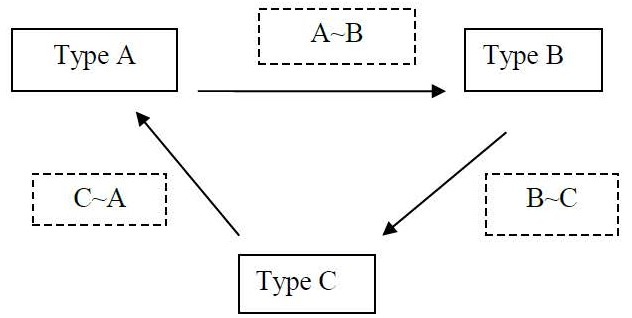
\includegraphics{figures/Croft1991_figure.jpg}
	\caption{Graphic representation of the NEC, adapted from \citet{Croft1991}.} \label{figure:nec1991}
	\begin{tikzpicture}
	  \node(center){};
	  \node at (30:2cm)  (b) [draw,rectangle]{Type B};
	  \node at (90:1.5cm) (ab) [draw,rectangle,dashed]{A{\textasciitilde}B};
	  \node at (150:2cm) (a) [draw,rectangle]{Type A};
	  \node at (210:1.5cm) (ca) [draw,rectangle,dashed,rotate=0]{C{\textasciitilde}A};
	  \node at (270:2cm) (c) [draw,rectangle]{Type C};
	  \node at (330:1.5cm) (bc) [draw,rectangle,dashed,rotate=0]{B{\textasciitilde}C};
	  \draw[-Latex](a) -- (b);
	  \draw[-Latex](b) -- (c);
	  \draw[-Latex](c) -- (a);
	\end{tikzpicture}

\end{figure}\noindent

The graphic representation of the cycle may lead to the impression that the stages outlined in it are necessarily sequential. \citet[22]{Croft1991} states very clearly that this is not the case; in fact, overlaps of different stages are expected. The comparative data compiled in the last ten years provide ample support for this generalization, see \citet{Veselinova2016} as well as several chapters in this book for instance \citet{chapters/Wilmsen_Arabic,chapters/Oreal_AncientEgyptian,chapters/Lam_Chinese}, to name a few.

Croft views the evolution of general negation markers from negative existentials as a grammaticalization process that involves instantiations of several commonly observed processes such as fusion, emphasis and its subsequent loss, competition/co-existence of different different encodings for one and the same function, as well as analogy. Fusion between a negator and a positive existential results in a special negative existential. Once created, negative existentials can expand their domain of use in different ways. One is by being added as emphatic elements to negated verb constructions. This kind of development is extensively discussed in this volume as well (\citealt{chapters/Bantu-Bernander-Devos-Gibson,chapters/Guillaume_Tacana,chapters/Intertwining-Auwera-Krasnoukhova-Vossen}), see also the discussion of negative existentials commonly used as negative answer words \textit{No} in \sectref{sect:negex}. Another pathway of expansion, outlined by \citet{Croft1991}, is that a negative existential can take over the negation of a specific tense-aspect-mood category in the domain of verbal negation. This creates variation in the domain of standard{\slash}verbal negation. Gradually, a negative existential, which is already used in a particular sub-domain of standard negation, can expand to negate all verbal predications. The cycle is considered to have gone full circle when the erstwhile special negative existential has started to be used together with the affirmative one for the negation of existential predications. In other words, there is a new, single negation strategy used both in verbal and in existential predications.


\citet[23--24]{Croft1991} notes that the NEC is productive in languages where predicate concatenation is possible and that the morpho-syntactic characteristics of specific languages may inhibit or halt the cycle. These generalizations are further confirmed and expanded in this volume (cf. discussion in \sectref{sec:intro:3}). Croft closes his article by stating that the dynamicization of typological data is highly significant for performing historical language studies since in many cases contemporary language data is all we have access to. At the same time, he does emphasize that models based on dynamic typology should be tested by the historical-comparative method whenever possible. This is what many of the authors of this book have done. The detailed datasets from specific families or language clusters allow for testing of the model in a fine-grained manner; in addition some authors, e.g. \textcitetv{chapters/IEUR-Verkerk-Shirtz} have also used statistical procedures for simulating a possible historical evolution.

\section{Outline of the topics covered in this book} \label{section:outline_of_topics}\label{sec:intro:3}
The topics discussed in the book follow several general directions. These include
(i) the interaction of negative existentials with SN, which in terms of the NEC implies an analysis of comparative data in terms of its different stages;
(ii)  the duration of different stages together with hypotheses about the time required for a completion of the NEC;
(iii) the constructions or processes that commonly contribute to negative existentials entering the verbal domain;
(iv) a topic raised by several authors is situating the NEC among other cycles and the general theory of cyclical developments in language change;
(v) finally, other special negators, not just negative existentials have been noted to undergo similar processes.

The interaction of the negative existentials with standard negation is manifested in the cross-linguistic frequency of specific stages of the NEC and the co-occurrence of the stages with one another.

The following can be said about the frequency of occurrence of the types outlined in the original model \citep{Croft1991}. The studies in this volume confirm the results of earlier findings (e.g. \citealt{Croft1991,Veselinova2014,Veselinova2016}): Type B, see (\ref{ex:ritharrngu1}), (Ritharrngu) is cross-linguistically very common and Type A, illustrated in (\ref{ex:odam1}), O'dam, is also widely attested, while Type C, see (\ref{ex:tongan1}), Tonga, is the rarest. Since the attestations or reconstructions of changes from one type to another are essential for the detection of a cyclic development, the inspection of transitional types forms a central part of the volume. Moreover, the transitional types seem to be more common than the stable types A, B and C. Especially attestations of A{\textasciitilde}B, (\ref{ex:tajik1}), Tajik, and B{\textasciitilde}C, (\ref{ex:mandarin1}), Mandarin, are found in many languages and families, whereas C{\textasciitilde}A, (\ref{ex:gaozhou1}), Gaozhou, is encountered more seldom. This can be seen as further evidence for the observation that the transitional stages A{\textasciitilde}B and B{\textasciitilde}C tend to arise relatively easily and to be relatively stable, whereas C{\textasciitilde}A (and the Type C itself) seem to pass more rapidly. In other words, contextually restricted negative existentials appear to develop easily; likewise, it is cross-linguistically common for negative existentials to be involved in partial take-overs of verbal negation. Thus the stages with variation appear to be both cross-linguistically common and diachronically stable as they can be demonstrated to last for extended periods of time, see data from Old Egyptian \parencitetv{chapters/Oreal_AncientEgyptian} as well from Arabic varieties \parencitetv{chapters/Wilmsen_Arabic}.

As pointed out by \citet{Croft1991} and also \citet{Veselinova2016}, types or stages of the cycle need not be sequential. In fact, it is cross-linguistically common for different stages to be present in a language simultaneously. The data in this book provide ample illustrations for this statement. For instance, \textcitetv{chapters/Lam_Chinese} demonstrates that the negative existential function of the predicate \textit{méi} (Type B in the NEC) and its uses as a general verbal negator (Type B{\textasciitilde}C in the NEC) emerged in Mandarin roughly at the same time, see data in (\ref{ex:mandarin2}) below.

\begin{exe}
\ex Mandarin [cmn] \parencitetv{chapters/Lam_Chinese} \label{ex:mandarin2}
\begin{xlist}
\ex \textit{méi} as a negative existential \label{ex:mandarin2a}\\
{\cn 一向都\textbf{沒}分別}\\
\gll yixiang dou \textbf{mei} fenbie\\
 along all \textbf{\textsc{mei}} difference\\
 \glt `There's no difference all along.' ({\cn 《朱子語類》}\emph{Zhuzi Yulei} AD 1270)\\

\ex \textit{méi} as verbal negator \label{ex:mandarin2b}\\
{\cn 都\textbf{沒}理會了}\\
\gll dou \textbf{mei} lihui le\\
  all \textbf{\textsc{mei}} take.notice le\\
  \glt `[they] all didn't take notice.' ({\cn 《朱子語類》}\emph{Zhuzi Yulei} AD 1270)

\end{xlist}
\end{exe}

An interesting example of synchronic co-occurrence can be seen in Tacana \parencitetv{chapters/Guillaume_Tacana} where the Types A and B{\textasciitilde}C co-occur, something that is cross-linguistically rare. This co-existence of two types is due to the fact that the language has three different SN constructions whose use partly depends on the finiteness versus non-finiteness of the predicate verb. The three SN constructions are as follows
(i) bi-partite \textit{aimue}…\textsc{verb}=\textit{mawe}{\slash}\textit{mue};
(ii) \textit{aimawe}{\slash}\textit{aimue};
(iii) a proclitic \textit{mué=}.  The bi-partite construction \textit{aimue}…\textsc{verb}=\textit{mawe}{\slash}\textit{mue} can be used for the negation of both finite and non-finite predicate verbs as well as in existential clauses; this motivates postulating Type A for Tacana. The form \textit{aimawe} can not only be used as a single predicator to encode negative existence but also for the negation of non-finite verbs. Hence the postulation of Type B{\textasciitilde}C in the language. The proclitic \textit{mué=} is used for the negation of non-finite predicate verbs (\textit{mué=}...\textsc{v}[be/do-\textsc{infl}]) but not for existential predications.

\begin{exe}
\ex Tacana [tna] (\citetv{chapters/Guillaume_Tacana}) \label{ex:tacana1}
\begin{xlist}
\ex \label{ex:tacana1a}
\gll  \textbf{Aimue} =da ema \textbf{\uline{e}}-siapati-yu=\textbf{mue}.\\
\textsc{neg} \textsc{=prt} \textsc{1sg} \textsc{fut}-come\_back-\textsc{iter=neg}\\
\glt `Ya no voy a regresar.' na191\\ 
`I'm not going to come back again anymore.'

\ex \label{ex:tacana1b}
\gll {\ob}Da tiempo{\cb} \textbf{aimue} sapato ani-ina\textbf{=mawe}.\\
that time \textsc{neg} shoe sit-\textsc{hab.pst=neg}\\
\glt `En ese tiempo no había zapato.' ci024\\
'At that time, there were no shoes.'

\ex \label{ex:tacana1c}
\gll Kwati =mu \textbf{aimue} =tsu'u.\\
firewood =\textsc{cntr} nonexistent =\textsc{still}\\
\glt `La leña todavía no hay.' ci104\\
`There is no firewood yet.' (lit. firewood was nonexistent)

\ex \label{ex:tacana1d}
\textit{Biame \textbf{aimue} =da \textbf{dia} \textbf{a-ta-ina}}.\\
on\_the\_contrary \textsc{neg} \textsc{=prt} eat do\textsc{-3A-hab.pst}\\
\glt `Pero no lo comió.' qu004\\
`But (the jaguar) would not eat it.'

\ex \label{ex:tacana1e}
\gll \textbf{Mué=}pa \textbf{teje-ti-yu} \textbf{a-ta-idha} {\ob}jida mesa e-wane{\cb} beu.\\
\textsc{neg=rprt} find-\textsc{go-iter} do\textsc{-3A-rem.pst} that \textsc{3sg.gen} \textsc{npf}-wife \textsc{prt}\\
\glt `Dice que no lo ha ido hallar ese su mujer.' os043\\
`He didn't find his wife.'

\end{xlist}
\end{exe}
The data from Tacana show that stages which are distant from each other in the NEC model may persist simultaneously in a language. This can be seen in Arabic, too, where the so-called \textit{šī}-cycle has skipped stage B but exhibits the transitional stage B>C \parencitetv{chapters/Wilmsen_Arabic}.

It should be noted that the realization of the NEC is far from universal. There are languages and language groups that seem to have adhered to a single negation strategy, that is Type A, for long periods of time, with no detectable or very rare interaction between negative existence and SN. For the languages of this volume this is noted, for instance for a large part of the Bantu family\parencitetv{chapters/Bantu-Bernander-Devos-Gibson} and also for Romance languages \parencitetv{chapters/IEUR-Verkerk-Shirtz} that mostly adhere to Type A. In the case of Bantu, there are non-verbal constructions for the expression of negative existence, but these are only used in a regionally restricted set of languages. Moreover, negative existentials seem to have become standard negative markers mostly in language varieties that are heavily influenced by contact. In the Chadic languages, as well, Type A prevails \parencitetv{chapters/Chadic-Butters}. Another rather clear example where standard and existential negation do not seem to have interacted with each other is O’dam and likely South Uto-Aztecan \parencitetv{chapters/O_dam-Everdell-GarciaSalido}.

Several of the articles  shed light on the duration of the cycle of the NEC since they examine the extended time-depth of languages that have a very long written tradition. Such languages include Arabic, Ancient Hebrew, Ancient Egyptian and Chinese. As shown by \textcitetv{chapters/Lam_Chinese}, for example, several rounds of completion of the NEC can be detected in the evolution of negation from Old Chinese to modern Mandarin and Cantonese.

The examinations of the languages with a long written tradition confirm the earlier views that especially the transitional stages of the NEC tend to endure over long periods of time. Moreover, synchronic variation, tolerance of multiple constructions and overlap of different stages seems to be more common than a strictly consecutive succession of clearly definable stages of the cycle. This is often due to a condition where a new cycle was (re)started before the previous one was completed. For example, in Old Chinese more than ten different negative markers have been attested, at least three of which could be used in the negation of existence (see \citetv{chapters/Lam_Chinese}). Likewise, tolerance of multiple constructions, synchronic variation of older and emergent forms and overlap of stages are detected in Ancient Egyptian \parencitetv{chapters/Oreal_AncientEgyptian} and Ancient Hebrew \parencitetv{chapters/Hebrew-Naude-Miller-Wilson}.

It has to be pointed out, however, that written languages are often conservative and possibly do not represent actual language use. This is suspected, for example, by \textcitetv{chapters/Oreal_AncientEgyptian} in the case of Ancient Egyptian and \textcitetv{chapters/Wilmsen_Arabic} in the case of Arabic. In Arabic, the longest surviving existential negator \textit{laysa} has reached the stage C>A but the negator has mainly persisted in the conservative written language, whereas in speech it is only maintained in some dialects.

As stated in the conclusion of  \sectref{sec:intro:2.6}, Croft brings up analogy as one the driving factors that contribute to the spreading of the negative existential construction to another domain, such as the domain of verbal negation. This is also confirmed by studies in this volume, e.g. \textcitetv{chapters/Hebrew-Naude-Miller-Wilson} who discuss data from Ancient Hebrew. In this language  participial constructions, some of which included the negative existential, spread to the main predicate position. This in turn led to the reanalysis of the negative existential as the more general negator.

A major pathway whereby negative existentials enter the domain of verbal negation is their use with non-finite forms of the lexical verb. In the Nanaic languages discussed by \textcitetv{chapters/tungusic},
% \todo{This prints in a very odd way. I would like the citation to include the names of the authors, Oskolskaya and Stoynova (this volume)}
negative existentials are commonly used with a converb that also encodes simultaneous action, as illustrated in (\ref{ex:naikin-nanai1}) below.

\begin{exe}
\ex Naikin Nanai [gld] (\citetv{chapters/tungusic} citing \citet[209, text]{avrorin1986a}\label{ex:naikin-nanai1})\\
\gll Əǯi-ni sənə-m=də̄ aba.\\
husband-\textsc{3sg} wake.up-\textsc{cvb.sim.sg=emph} \textsc{neg.ex}\\
\glt `Her husband hasn’t woken up (lit. her husband is absent while waking up).' 
\end{exe}
In literal terms, the action encoded by the lexical verb in (\ref{ex:naikin-nanai1}) is seen as simultaneous with the state of absence predicated by the negative existential. The latter is subsequently reanalyzed as a negator for the action expressed by the lexical verb. The material presented by \textcitetv{chapters/tungusic} outlines different degrees of the conventionalization of such constructions in the Nanaic languages. The more conventionalized they become, the closer the negative existential comes to a general verbal negator.

Negative existentials are used with non-finite, nominalized forms of the lexical verb in many different languages around the world, see (\ref{ex:egyptian1}) below for an example.

\begin{exe}
\ex Ancient Egyptian [egy] (\citetv{chapters/Oreal_AncientEgyptian}) \label{ex:egyptian1}\\
\gll ni m{\ꜣ}=j mjtj n zrw pn\\
	\textsc{neg} see\textbackslash\textsc{nmlz=1sg} like of goose this\\
	\glt ‘I haven’t seen the like of this goose ever.’ (lit. ‘There is not my seeing the like of this goose’) (Meir III)

\end{exe}
As illustrated in (\ref{ex:egyptian1}), the action of seeing is negated by being conceptualized as a non-existent entity. Such uses of negative existentials present a clear pathway for them to expand into the domain of verbal negation. Several authors in this book highlight the functional and pragmatic motivation for this phenomenon.

For instance, \textcitetv{chapters/Oreal_AncientEgyptian} based on data from Ancient Egyptian, considers negative existentials as predicators of absence rather than operators of negation. When they combine with an action, the action itself is perceived as a wholesome object, hence the motivation for a nominalized verb form.

\textcitetv{chapters/Lam_Chinese} contributes to the understanding of the NEC in several different ways. The one relevant here concerns the use of SN markers and the negative existential with different verb classes in Hong Kong Cantonese. Lam points out that in this variety, activity predicates can be negated by either the SN marker \textit{mau4} and the negative existential \textit{mau5}. However, the SN marker \textit{mau4} and the negative existential \textit{mau5} are in complementary distribution with all other verb classes. Specifically, the SN marker \textit{mau4} is preferred with states, while the negative existential \textit{mau5} is preferred with accomplishments, achievements and semelfactives. All of these can be easily conceived of as entities. Thus Lam concludes that negative existentials in Chinese varieties are not negators for a specific tense-aspect category such as the perfect, as is often stated in grammars. Rather, negative existentials assert the non-existence of entities with varying degrees of abstraction, from very specific to very abstract objects. This in turn leads to them being re-interpreted as more general verbal negators.

\textcitetv{chapters/Australian-Phillips} presents data from several Australian families and demonstrates convincingly that privative markers, in many of them also the negative existentials, predicate the absence of things/entities. When used with words that encode actions, the privatives/negative existential predicate the non-actualization of events.

Negative existentials are frequently used as negative answer words \textit{No}, see (\ref{ex:intro:swahili-2}) from Swahili below (see also \sectref{sect:negex}).
\begin{exe}
\ex Swahili (G42) [swh] (\citetv{chapters/Bantu-Bernander-Devos-Gibson} citing \citet[25]{KingeiNdalu2009}) \label{ex:intro:swahili-2}
\begin{xlist}
\ex \label{ex:intro:swahili-2a}
\gll Ha-pa-na m-tu a-si-ye-fanya ma-kosa\\
\textsc{neg}-\textsc{sm}16-\textsc{com} 1-person
1-\textsc{neg}-\textsc{rel}1-make 6-mistake\\
\glt `There is no person who does not make mistakes.'
\ex \label{ex:intro:swahili-2b}
\gll U-na-kwenda Bagamoyo? Hapana.\\
	\textsc{sm.2sg}-\textsc{prs}-go Bagamoyo no\\
\glt 	`Are you going to Bagamoyo? No.'
\end{xlist}
\end{exe}


Such uses  emerge as another cross-linguistically common pathway whereby negative existentials expand into the domain of verbal negation, see for instance \textcitetv{chapters/Bantu-Bernander-Devos-Gibson}, \textcitetv{chapters/Moksha-Hamari}Hamari on Moksha, \textcitetv{chapters/Guillaume_Tacana} on Tacana and \textcitetv{chapters/Intertwining-Auwera-Krasnoukhova-Vossen} for a cross-linguistic perspective.

There are several possible pathways whereby negative answer words \textit{No} can be re-analyzed as more general markers of verbal negation. As discussed by \textcitetv{chapters/Bantu-Bernander-Devos-Gibson}, such words are frequent and salient and in situations of contact between speakers of different varieties, they can be easily re-analyzed as a general negator. This is the case of Standard Swahili in contact with other pidgin varieties of Swahili and also with other Bantu languages. Specifically, the Standard Swahili negative existential \textit{hapana} has been borrowed and integrated into their negation systems. For instance, in Pogolo, shown in (\ref{ex:pogolo1}) below, the word \textit{hapana} has become a bound prefix, much like many other expressions of SN in Bantu languages.

\begin{exe}
\ex Pogolo (G51) [poy] \parencitetv{chapters/Bantu-Bernander-Devos-Gibson}\label{ex:pogolo1}\\
\gll hapa-tu-hemer-a\\
	\textsc{neg-sm1pl}-buy-\textsc{fv}\\
\glt 'we are not buying'
\end{exe}

Another pathway whereby negative existentials/negative answer words \textit{No} become general negators is via their uses as sentence-external, pleonastic negators. Such a case is discussed, for instance by \textcitetv{chapters/Guillaume_Tacana} based on data from Tacana. In this language the word \textit{aimawe} is observed as a pleonastic negator as in \REF{ex:tacana2} below and also as a first element in one of the SN constructions, cf. (\ref{ex:tacana-1}).

\begin{exe}
\ex Tacana [tna] (\citetv{chapters/Guillaume_Tacana}) \label{ex:tacana2}
\judgewidth{Mother:}
\sn[Mother:]{%
\gll Manuame-pe-ta-kwa  tse  ekwana.\\
    kill\textsc{-compl}-3A-\textsc{pot}  \textsc{maybe}  \textsc{1pl}\\
\glt  `¡(Tu padre) nos puede matar a toditos!' au064\\
 `(Your father) can kill us all!'}
\sn[Son:\hspace{\stretch{1}}]{%
\gll \textbf{Aimawe}!  Ema  ebiasu  tuche-da.\\
    no  1\textsc{sg}  a\_lot  strong-\textsc{asf}\\
\glt  `No, yo tengo más fuerza que él.'\\
 `\uline{No} (he can't kill us)! (Because) I'm stronger (than him).'}
\end{exe}
\textcitetv{chapters/Guillaume_Tacana} reasons that \textit{aimawe}, which with all likelihood originates from a negative existential, is also commonly used as a negative answer word \textit{No}. This use leads to the one as a pleonastic negator, external to the proposition. In many situations, the sense of emphasis is lost and \textit{aimawe} is re-interpreted as the initial part of a bi-partite SN construction with a reduced form \textit{aimue}. In essence, \textcitetv{chapters/Guillaume_Tacana} outlines a development highly reminiscent of a Jespersen Cycle.

This brings us to another important topic of the book, namely situating the NEC among other well known cycles. Authors such as van der Auwera, Krasnoukhova and Vossen as well as van Gelderen cast the NEC in a theoretical perspective together with providing a discussion about differences and similarities between different cyclical processes with a special focus on those that produce some kind of negative marker. These authors make significant contributions to the volume and to the theory of cycles. For the purposes of this summary, we focus on one, namely the interaction between NEC and Jespersen Cycle.

Van der Auwera, Krasnoukhova and Vossen provide a generalized definition of the notion of Jespersen Cycle. Specifically, they define it as a process where the SN marker co-occurs with another element α which can be either non-negative like French \textit{pas} or negative like Swedish \textit{inte}. This collocation may result in an univerbation or the non-negative element may become negative by contamination and may eventually oust the original SN marker. After an analysis and a refined definition of the NEC, these authors consider possible parallels and also any possible interaction between the Jespersen Cycle and the NEC. To highlight this aspect, they bring up Mara, a Pama-Nyungan language from Northern Australia and Wintu, an extinct language, formerly spoken in northern California. Both of these languages are discussed by \citet[10, 14]{Croft1991} but van der Auwera, Krasnoukhova and Vossen provide a new interpretation to these data. Specifically, these authors highlight the fact that negative existentials, when used as pleonastic negators, can produce emphatic negative constructions where the negative elements are in fact doubled as in Tacana, (\ref{ex:tacana2}). The occurrence of such constructions and the subsequent loss of the sense of emphasis is strongly reminiscent of a Jespersen Cycle development. The authors point out that this has been implicitly stated by \citet[14]{Croft1991}. In their contribution they make it more explicit and also provide a cross-linguistic perspective suggesting that this pathway for negative existentials to enter the domain of verbal negation is much more common than shown by previous research.


The interaction of the NEC and Jespersen Cycle is also mentioned by some other authors of the volume. \textcitetv{chapters/Bantu-Bernander-Devos-Gibson} make a cautious observation of a possible beginning of the Jespersen Cycle in which a negative existential is involved in certain Bantu languages: in these languages, there are discontinuous constructions for standard negation where the inherited preverbal standard negator is accompanied by a postverbal negative particle which is identical with the existential negator. Such a construction is attested in Iyaa, illustrated in (\ref{ex:iyaa1}).


% \todo{protectedex does not seem to work: the whole example shifts to the right}%\protectedex{
\begin{exe}
\ex Iyaa (B73c) [iyx] (\citetv{chapters/Bantu-Bernander-Devos-Gibson} citing  \citet[439, 436]{Mouandza2001}) \label{ex:iyaa1}
\begin{xlist}
\ex standard negation \label{ex:iyaa1a}\\
\gll ndé a á-yěne pé ku mu-s{\'\i}ti\\
	\textsc{pers}1 \textsc{neg} \textsc{sm}1-go.\textsc{pfv} \textsc{neg} 17 3-forest\\
\glt `He has not gone to the forest.' 

\ex negative existential \label{ex:iyaa1b}\\
\gll b{\`a\`a}t\`a pé\\
	2.person \textsc{neg}\\
\glt `There are no people.'
\end{xlist}
\end{exe}
%}
 Furthermore, a possible involvement of a negative existential in a Jespersen Cycle type of an evolution of negation is also discussed in the case of Arabic \parencitetv{chapters/Wilmsen_Arabic}, Ancient Egyptian \parencitetv{chapters/Oreal_AncientEgyptian}, Nanai \parencitetv{chapters/tungusic} and Tacana \parencitetv{chapters/Guillaume_Tacana}, see also \textcitetv{chapters/Othercycles-Gelderen} for a formal perspective on this topic.
  
 Van Gelderen considers the NEC in the context of several other cyclical processes such as the Jespersen Cycle, the Givón Cycle, whereby verbs with referential content are shown to evolve into negation markers and, finally, the Copula Cycle. In her view, negative existentials and, subsequently, the NEC are restricted to verbs that represent univerbations between a negator and another item. Lexical sources for negative existentials or negators are considered a separate development, which she includes in the Givón Cycle. Van Gelderen grounds her discussion in formal syntax with an abundance of cross-linguistic data. The issues she highlights include the source verbs for the NEC, its verbal nature, as opposed to the nominal nature of the Jespersen Cycle, and finally, similarly to other authors in this volume, the possibility of doubling the negative maker in constructions produced by the NEC. Ultimately, she also brings up factors that can facilitate the operations of cycles such as the NEC and the Givón Cycle. Namely, she points out that the realization of these cycle is most likely when the source verbs are not specified for too many features.
 
 Finally, as discussed in \sectref{section:ascriptiveneg} and \sectref{section:stative-negators}, several scholars, notably, Baranova and Mishchenko as well as Wilmsen and van Gelderen stress the fact that other special (non-standard) negators may expand into the domain of standard negation via processes similar to the NEC, e.g. via creation of emphatic constructions, co-existence of stages with variation, restriction to a specific verbal category for periods of time of varying length. Thus the cycle dubbed Negative Existential Cycle need not be restricted to negative existentials only.

\section{Notions central to this book}\label{sect:notions}\label{sec:intro:2}
\subsection{Standard negation}\label{sect:sn}\label{sec:intro:2.1}
The term \textsc{standard negation} covers negation strategies used in main declarative clauses with an overt lexical verb, see Miestamo (\citeyear[1]{Miestamo2005}) who follows \citet{payne1985a} in keeping this term for the negation of verbal predications. As noted by Dahl (\citeyear[10--11]{Dahl2010}), the term is not entirely felicitous as it implies that all other negation strategies are somehow “non-standard”, and it is not at all clear that it should be so. In defense of the term \textit{standard negation}, it should be pointed out that frequently, though not always, the negation strategy used to negate verbal predications is also pragmatically the most neutral one in many languages. Since the essence of  SN is the negation of verbal predications, many authors in this book use the terms \textit{standard negation} and \textit{verbal negation} interchangeably.

There is a strong tradition in the scholarship of negation to contrast affirmative and negative constructions. \citet[6--7]{Miestamo2005} introduces an important distinction between symmetric and asymmetric negation. Symmetric negation refers to cases when the negative construction differs from the affirmative by one added element\footnote{The negative element itself may comprise several parts, like French \textit{ne} \textsc{verb} \textit{pas}.}. Asymmetric negation involves changes in the affirmative construction that are more complex than the mere addition of an element. One of Miestamo’s major contributions to the typology of negation is the outline of several different types of asymmetries between affirmative and negative constructions. One of them, asymmetry according to finiteness, is especially relevant for the NEC.

SN in Moksha in (\ref{ex:moksha-1a}-\ref{ex:moksha-1b}), is considered symmetric as \textit{af moran} in (\ref{ex:moksha-1b}) differs from \textit{moran} in (\ref{ex:moksha-1a}) only by the negative particle \textit{af}. However, negation in categories other than the indicative non-past can be asymmetric in that a special negative auxiliary is used and the lexical verb has to appear in a special form dubbed connegative in Uralic linguistics, cf. (\ref{ex:moksha-2a}-\ref{ex:moksha-2c}). There are two kinds of asymmetry we observe in these data:
(i) constructional asymmetry, as different kinds of constructions are used in the affirmative and the negative domains and
(ii) asymmetry according to finiteness, since the lexical verb from the affirmative appears in a non-finite form in the negated proposition.

\begin{exe}\ex Moksha [mdf] \parencitetv{chapters/Moksha-Hamari} \label{ex:moksha-2}
\begin{xlist}
\ex \label{ex:moksha-2a}
\gll morɑ-ń\\
sing-\textsc{pst1.1sg}\\
\glt ‘I sang'
\ex \label{ex:moksha-2b}
\gll iź-ǝń morɑ\\
\textsc{neg.pst}-\textsc{pst1.1sg} sing.\textsc{cng}\\
\glt ‘I did not sing’
\ex \label{ex:moksha-2c}
\gll ɑš-ǝń morɑ\\
\textsc{neg.pst}-\textsc{pst1.1sg} sing.\textsc{cng}\\
\glt ‘I did not sing’
    
    
\end{xlist}

\end{exe}
As indicated in (\ref{ex:moksha-1d}--\ref{ex:moksha-1e}), the auxiliary \textit{ɑš}- used in (\ref{ex:moksha-2c}) actually developed from the negative existential in Moksha. This brings us to introducing definitions of existential predications, \sectref{sect:existentials}, and negative existentials, \sectref{sect:negex}.

\subsection{Existential sentences}\label{sect:existentials}\label{sec:intro:2.2}
The term \textsc{existential sentence} was introduced in modern linguistics by Otto Jespersen (\citeyear[154--156]{jespersen1924}). He begins by contrasting sentences such as (\ref{ex:jespersen-1}) and (\ref{ex:jespersen-2}) as possible openings of a story and notes that (\ref{ex:jespersen-2}) is a much more natural way to begin a story than (\ref{ex:jespersen-1}).

\begin{exe}\ex
    \label{ex:jespersen-1}
          A tailor was once living in a small house. \citep[154]{jespersen1924}
    \end{exe}
    
\begin{exe}\ex
    \label{ex:jespersen-2}
          Once upon a time there was a tailor. \citep[154]{jespersen1924}
    \end{exe}
By highlighting the story opening function of (\ref{ex:jespersen-2}), Jespersen pinpoints what would later be identified as one of the most important discourse functions of these constructions, namely, introducing a new referent into the discourse. Jespersen goes on to discuss a number of well-known structural features of existential clauses: use of an expletive locative pronoun such as \textit{there} in English, a lexical item with odd characteristics in a predicate position, indefinite subject in a non-prototypical position, inverse word order. Jespersen’s explicit definition of existential sentences as [sentences] “in which the existence of something is asserted or denied” has been criticized as too general and weak, \citep[212]{McNally2016}. However, he has to be credited with delimiting these sentences as a separate construction type with specific functions and identifiable formal properties.

Since Jespersen (\citeyear{jespersen1924}), an enormous amount of scholarly work has been devoted to existential constructions, though many of them simply take the notion for granted, (see also \citet[43-44]{creissels2019} and \citet{haspelmath2021} for detailed discussions of this issue). In what follows we summarize selected lines of research that have helped shape the understanding of existential constructions as it appears in this book. They include the close link between location, existence and possession, the terminology used for the analysis of existential constructions, their semantics and functions and, finally, their structural encoding.

\subsubsection{Location, existence and possession}\label{sect:loc-ex-poss}\label{sec:intro:2.2.1}
A number of studies have been devoted to highlighting the conceptual link between location, existence and possession, see (\citealt{lyonsPossession1967,Clark1978,bickertonRootsLanguage1981,Heine1997,koutevaWorldLexiconGrammaticalization2019,Koch2012}); the list provided here is not exhaustive). Such a link is illustrated by Finnish in (\ref{ex:finnish-1}). In this language, the located argument appears in the nominative case, the verb \textit{olla} ‘be’ agrees with it in person and number and the locative phrase is marked by one of the locative cases, typically though not always, the adessive or the inessive, see (\ref{ex:finnish-1a}). In existential predications, see (\ref{ex:finnish-1b}), the same arguments are observed but the word order is different in that the locative phrase occurs in the theme. Finally, possessive predications, (\ref{ex:finnish-1c}), use the same template as existentials in that the possessor is marked by a locative case, the adessive. It has to be pointed out that the case marking of arguments in this construction is complicated. The case marking is the same (nominative) in locative and existential sentences only if the subject is singular and the sentence is affirmative. With a plural or mass noun subject or under negation, the subject of existential and possessive sentences is in the partitive (see \ref{ex:finnish-1c}).

\begin{exe}
\ex Finnish [fin] \citet[113]{vilkunaPredicativePossessionClause2020} modified by Arja Hamari\label{ex:finnish-1}
\begin{xlist}
\ex \textsc{locative}\label{ex:finnish-1a}\\
\gll Koira on sohva-lla {\slash}Anna-n syli-ssä.\\
dog be.\textsc{prs.3sg} sofa-\textsc{ade} {\slash}Anna-\textsc{gen} lap-\textsc{ine}\\
\glt ‘The dog is on the sofa / Anna’s lap.’

\ex \textsc{existential}\label{ex:finnish-1b}\\
\gll Sohva-lla {\slash}Anna-n syli-ssä on koira {\slash}koir-i-a.\\
sofa-\textsc{ade} {\slash}Anna-\textsc{gen} lap-\textsc{ine} be.\textsc{prs.3sg} dog{\slash}dog-\textsc{pl}-\textsc{par}\\
\glt ‘There is a dog {\slash}are dogs  on the sofa {\slash}Anna’s lap.’

\ex \textsc{possessive}\label{ex:finnish-1c}\\
\gll Anna-lla on koira {\slash}koir-i-a {\slash}raha-a.\\
Anna-\textsc{ade} be.\textsc{prs.3sg} dog {\slash}dog-\textsc{pl}-\textsc{par} {\slash}money-\textsc{par}\\
\glt ‘Anna has a dog / dogs / money.’
\end{xlist}
\end{exe}
Thus in Finnish, the introduction of a new participant in the discourse is expressed by placing it in a particular location or context. As has been noted by many authors, and likewise in the articles of  this book, the locational scheme is pervasive for the encoding of existential predications, (see also pertinent data in \sectref{sec:intro:2.2.4}). In fact, there are authors such as \citet[1]{creissels2019} who focus exclusively on what he calls \textit{inverse-locative predications}, that is, predications such as \textit{There is a book on the table}. For him a defining feature of existential predications is “the perspectivisation of the relationship [...] from ground to figure”; as this author points out, figure-ground relationships are also encoded by plain locational sentences such as English \textit{The book is on the table} \citep[41]{creissels2019} but the perspective of novelty is missing. \citet{dryer2007a} offers a more general perspective on these constructions, which we also adopt here, see \sectref{sec:intro:2.2.3}. In particular, Dryer highlights the fact that existential constructions, regardless of whether they specify a location or not, introduce a new referent into the discourse.

\subsubsection{Terminology used in the analysis of existential predication}\label{sect:terminology}\label{sec:intro:2.2.2}
Several important notions used for the analysis of existential predications follow studies set in generative semantics and syntax. In a number of works, for example in  \citet[1]{BentleyCiconte2013} who follow \citet{Francez2011,McNally2011} and \citet{Francez2007}, it is pointed out that the noun phrase in existential constructions\footnote{The terms \textit{predication} and \textit{construction} are used synonymously here.} is a non-prototypical subject and it is identified as a \textit{pivot}. Furthermore, many authors argue that noun phrases in existential constructions are indefinite and either generic or non-specific, see \citet[219]{McNally2016} and also \citet[538]{Koch2012} for examples. \citet[1--2]{BentleyCiconte2013} note that the pivot is the only obligatory component in an existential construction while any other components are optional. The optional components include the locative phrase, the expletive pronoun and the verb form, these authors label \textit{existential copula}. In many languages it can be a form of the verb ‘be’ as it is in English or in Finnish, as shown in (\ref{ex:finnish-1}) above. In other languages it can be a form dedicated to the existential constructions as the form \textit{hay} in Spanish, see (\ref{ex:spanish-1}).

\begin{exe}
\ex Spanish [spa] (constructed example)\label{ex:spanish-1}\\
\gll Hay queso en la nevera.\\
\textsc{ex}	cheese in \textsc{def} fridge\\
\glt \textquoteleft There is cheese in the fridge.’
\end{exe}
It has to be said that there is still no consensus on the terminology used for the verb-like element that may be present in existential constructions. In addition to existential copula, it can be referred to as \textit{existential verb}, or \textit{existential particle} to name a few alternatives. The terminology used for this component can be very idiosyncratic but while not all authors make it explicit, the choice of denomination may be contingent on the degree of specialization of this element. For instance, forms such as those used in the English and Finnish existential constructions are referred to as copulas as they still belong to the paradigm of the verb ‘be’ in these languages. Conversely, the form \textit{hay} in Spanish is frozen in the existential construction and has only a diachronic connection to \textit{habere} ‘have’ from which it stems; \textit{hay} is often referred to as the existential verb or as existential particle. As the authors contributing to this book work in different schools and traditions, readers will find variation in the labeling of the verb-like element in existential constructions\footnote{\citet{haspelmath2021} suggests to dub this element existive. This term is yet to be established in future research.}. For the purposes of consistency in the glossing of the data, it is glossed as \textsc{ex} for ‘existential’.

\subsubsection{Semantics and functions of existential constructions}\label{sect:semantics-of-ex}\label{sec:intro:2.2.3}
\citet[240--243]{dryer2007a} discusses existential constructions as a separate clause type and illustrates it with examples from Ma’anyan, an Austronesian language spoken in Kalimantan, Borneo, Indonesia, see (\ref{ex:maanyan-1}).

\begin{exe} \ex Ma’anyan [mhy] (\citealt[240--241]{dryer2007a} citing \citealt{gudai1988})\label{ex:maanyan-1}
\begin{xlist}
\ex \label{ex:maanyan-1a}
\gll inehni naqan hang sungking\\
mother be.at at kitchen\\
\glt ‘his mother is in the kitchen’

\ex \label{ex:maanyan-1b}
\gll naqan erang kaulun wawey mawiney hang tumpuk yeruq\\
be.at/exist one \textsc{clsfr} woman beautiful at village the\\
\glt ‘there was a beautiful woman in the village’

\ex \label{ex:maanyan-1c}
\gll sadiq naqan tumpuk eteqen\\
olden.time exist village Eteen\\
\glt ‘once upon a time there was a village called Eteen’
\end{xlist}

\end{exe}
All three examples in (\ref{ex:maanyan-1}) above include a locative verb \textit{naqan} ‘be at, exist’ and a noun phrase whose location or existence are predicated. As discussed by \citet{dryer2007a}, the sentences in (\ref{ex:maanyan-1}) have similar components but differ in perspective and information structure. While (\ref{ex:maanyan-1a}) makes a statement about the location about an individual known to the participants, \textit{inehni} ‘his mother’, (\ref{ex:maanyan-1b}) presents an individual unknown to the hearer, \textit{erang kaulun wawey mawiney} ‘a beautiful woman’ at a specific location (\textit{hang tumpuk yeruq} ‘at the village’). The sentence in (\ref{ex:maanyan-1c}) introduces something new to the hearer, the existence of a village called Eteen. \citet[241]{dryer2007a} points out that the sentence in (\ref{ex:maanyan-1a}) can be characterized as a locative clause, while the sentence in (\ref{ex:maanyan-1b}) can be interpreted either as a locative or as an existential predication. Finally, (\ref{ex:maanyan-1c}) is characterized as existential only. At the same time, Dryer offers a very important analytical insight. Specifically, he points out that using the label \textit{existential} for clauses such as (\ref{ex:maanyan-1b}-\ref{ex:maanyan-1c}) is, in fact, misleading since their discourse function is to introduce participant(s)/facts new to the hearer\footnote{This is very close to Jespersen’s original understanding, which has been completely neglected when definitions of existential constructions have been offered.}. This accounts for the restriction to indefinite NPs as pivots and the fact that NPs in existential constructions are often generic.

It is also our understanding that clauses dubbed \textit{existential} are not merely about stating the existence of an entity in a philosophical sense as is sometimes suggested. Since the term \textit{existential sentence} is well established, we will keep it here too. But it has to be clear what it covers. The constructions we focus on here have a general communicative function in that they bring a novel entity into (a specific) context. This is commonly construed in terms of location or possession, (consult \sectref{sec:intro:2.2.4} for more data on this issue). 

Existential constructions are generally a feature of spoken registers. As has been pointed out already, in languages where existential constructions can be identified, they show a number of features which set them apart from other constructions as a separate construction type. It is important to bear in mind that a sentence such as (\ref{ex:hyparctic-1}) is an intransitive sentence and not an existential construction, in the specialized sense used here\footnote{\citet{haspelmath2021} suggests the term \textit{hyparctic} < Greek \textit{hýparxis} ‘existence’ to include such sentences as well. As his work has not been available to the authors of this book but to the editors only, we mention it for the sake of completeness.}.

\begin{exe}
\ex \label{ex:hyparctic-1}
Ghosts exist.
\ex \label{ex:existential-1}
There are ghosts in the forbidden forest.
\end{exe}
The existence of ghosts is stated in (\ref{ex:hyparctic-1}) but without the perspective of novelty and a figure-ground reversal present in (\ref{ex:existential-1}). Östen Dahl (p.c.) points out that it is most probably the case that intransitive verbs of existence such as English \textit{exist}, French \textit{exister}, Bulgarian \textit{съществувам/səshtestvuvam} ‘exist’ are typically present in languages with a long written tradition and largely restricted to formal registers. This statement is currently an informed hypothesis which should be empirically tested by future research (see \citet{olssonExistentialConstructionsConstructions2022} for a small-scale study of this issue). 

Several other points need to be mentioned about the semantics of constructions dubbed existential. They concern the functions commonly identified for the existential construction, the temporal stability of the predicated novelty{\slash}entity, the role of the locative phrase for the interpretation of the construction, the restriction to indefinite NPs{\slash}pivots and the productivity of the construction.

\citet{haspelmath2021}, in his quest to define a comparative concept for existential sentences, identifies the following functions: the indication of permanent presence, episodic presence and availability, see (\ref{ex:existential-functions-1}) for some examples.

\begin{exe}
\ex Functions commonly identified for existential constructions \citep{haspelmath2021}\label{ex:existential-functions-1}
\begin{xlist}
\ex \textsc{permanent presence} \label{ex:existential-functions-1a}\\
There are lions in Africa.
\ex \textsc{episodic presence} \label{ex:existential-functions-1b}\\
There is a knife on the table.
\ex \textsc{availability} \label{ex:existential-functions-1c}\\
There are oranges at the market.
\end{xlist}
\end{exe}

\citet[540]{Koch2012} makes a distinction between temporary location, dubbed by him \textsc{rhematic location} (\textsc{r-location}), (\ref{ex:somali-1a}), bounded existence, (\ref{ex:somali-1b}), and finally generic existence, (\ref{ex:somali-1c}). The distinction between bounded and generic existence is defined by the presence or absence of a locative phrase in the construction.
\begin{exe}
\ex Somali [som] \citet[540]{Koch2012} \label{ex:somali-1}
\begin{xlist}
\ex \label{ex:somali-1a}
\gll Miis-ka buug baa dul yaalla.\\
table-\textsc{def} book \textsc{foc} upon be.\textsc{3sg.m.prs}\\
\glt ‘There is a book on the table.’
\ex \label{ex:somali-1b}
\gll Libaax-yo badan baa jira’ Afrika.\\
lion-\textsc{pl} many \textsc{foc} exist.\textsc{prs} africa\\
\glt ‘There are many lions in Africa.’
\ex \label{ex:somali-1c}
\gll Dad badan oo madluumiin-a baa jira’.\\
people many \textsc{rel} unhappy-be \textsc{foc} exist.\textsc{prs}\\
\glt ‘There are many unhappy people.’

\end{xlist}
\end{exe}
\citet[238--240]{Koch2012} argues that in a sentence such as the one in (\ref{ex:somali-1a}) the location of a specific entity is predicated, while in sentences such as those in (\ref{ex:somali-1b}-\ref{ex:somali-1c}) the existence of a generic entity is predicated. In his discussion, Koch points out that in Somali different verbs are used: \textit{yalli}- in \textsc{r-locationals} and \textit{jiir} in constructions predicating existence. Expressions such as those in (\ref{ex:somali-1a}) correspond to what \citet{hengeveld1992} calls \textsc{locative-presentative} constructions. However, as noted by \citet{dryer2007a}, sentences such as those in (\ref{ex:maanyan-1b}) and (\ref{ex:somali-1a}) can be interpreted as either locative or as existential. What makes them functionally distinct from plain predications of location such as those in (\ref{ex:maanyan-1a}) is the fact that they introduce a participant new to the hearer. For detailed studies of existential predications, the distinction noted by \citet{Koch2012} is important and should be studied further, see examples from German in \REF{ex:german-1}. However, for the purposes of identifying specialized constructions that bring something new to the discourse, as (\ref{ex:somali-1a}) should be counted as existential together with (\ref{ex:somali-1b}--\ref{ex:somali-1c}). The presence or absence of a locative phrase, that is, binding the novelty to a specific location or  making it a general fact, has a minimal role for the information structure of these constructions.

The final point to consider relates to the properties of the pivot and the productivity of these constructions. As discussed in \sectref{sec:intro:2.2.2} above, many authors point out that in an existential construction the pivot has to be indefinite and either non-specific or generic. This would exclude pivots in constructions such as those in (\ref{ex:maanyan-1b}) and (\ref{ex:somali-1a}) as the pivots in these examples are clearly specific. In addition, the presence of a quantifier may contribute further to the individuation and the degree of specification of the pivot. However, as argued above, from a communicative point of view, these constructions do exactly the same job as the constructions with non-specific or generic pivots. There are authors such as \citet[242]{dryer2007a} who argue that constructions with a definite pivot such the one shown in (\ref{ex:the-dog})
% \todo{cross-reference not working, keeps referring to a section and not to the example below There is the dog in the garden}
are not to be considered existential and are, in fact, a different construction altogether.

\begin{exe}
\ex \label{ex:the-dog}
There is the dog in the garden
\end{exe}
The construction in (\ref{ex:the-dog}) points to a dog in the garden that is surely known to both speaker and hearer. In this sense, (\ref{ex:the-dog}) is clearly different from constructions with an indefinite pivot. However, sentences like (\ref{ex:the-dog}) are typically used to introduce a new turn\slash topic to the conversation. In that sense, we see them as an extension of the existential constructions. In other words, existential constructions can be productive; they show varying degrees of productivity in different languages.

\subsubsection{Structural encoding of existential constructions}\label{sect:existentials-structure}\label{sec:intro:2.2.4}
This section builds on \citet{McNally2016}, who in turn draws most of her material from \citet{Creissels2014}. As discussed in \sectref{sect:loc-ex-poss}, Creissels restricts his focus to inverse-locative constructions, and studies their encoding in a non-stratified sample of 256 languages\footnote{The amount of languages studied in \citet{creissels2019} is much larger, up to 700 languages. However, as Creissels (\citeyear[39]{creissels2019}) states, it is not a sample in a “technical sense” as there is no stratification.}. Although this is a large amount of material, it is safe to say that a well-designed quantitative study of the encoding of existential constructions is still in demand. Nonetheless, these authors outline several broad strategies for the encoding of existential constructions and to date these are the only cross-linguistic overviews available. \citet{McNally2016} presents four types of existential constructions which we list in Table \ref{tab:structural-types-EX-constructions} and also add a fifth type, not mentioned by any of these authors.

\begin{table}
\begin{tabular}{ll}
\lsptoprule
\textsc{Type 1} & Those with a special existential predicate  \\
\textsc{Type 2} & Those based on copula constructions\\
\textsc{Type 3} & Those based on possessive constructions\\
\textsc{Type 4} & Those based on expletive impersonal constructions\\
\textsc{Type 5} & Verbless predications with a predicate nominal only\\
\lspbottomrule
\end{tabular}
\caption{Structural types of existential constructions}
\label{tab:structural-types-EX-constructions}
\end{table}

These different encodings are further discussed and illustrated below.

\textsc{Type 1}:	Existential constructions with a special predicate, see Spanish in (\ref{ex:spanish-1}), Hausa in \REF{ex:hausa-1} and Turkish in \REF{ex:turkish-1} below. In these constructions, the linking element is an item dedicated to the existential construction. In most cases it is not used in locative predications with a definite subject.
\begin{exe}
\ex Hausa [hau] (\citetv{chapters/Chadic-Butters}, citing \citealt[178--179, 357]{Newman2000}) \label{ex:hausa-1}
\begin{xlist}
\ex \label{ex:hausa-1a}
\gll \textbf{àkwai} wani bā̀ƙō à kōfā̀ \\
  	\textsc{ex} \textsc{indf} stranger \textsc{prep} door\\
\glt `There is a stranger at the door.'

\ex \label{ex:hausa-1b}
\gll \textbf{dà} kuɗɪ̄\\
  	\textsc{ex} money\\
\glt `There is money.'

\ex \label{ex:hausa-1c}
\gll Inà gidā.\\
\textsc{1sg.cont} home\\
\glt `I am at home.'
\end{xlist}
\end{exe}

\begin{exe}
\ex \label{ex:turkish-1}Turkish [tur] \citep[44, 41]{vanschaaik1994}
\begin{xlist}
\ex \label{ex:turkish-1a}
\gll Su \textbf{var-dı}.\\
water exist-\textsc{pst}\\
\glt `There was water.'

\ex \label{ex:turkish-1b}
\gll Ev-de-ydi-k.\\
home-\textsc{loc}-\textsc{pst}-\textsc{1pl}\\
\glt `We were at home.'
\end{xlist}
\end{exe}

The examples from Hausa require some clarification. While \textit{àkwai} (\ref{ex:hausa-1a}) can be said to be a specialized existential predicate, \textit{dà} in (\ref{ex:hausa-1b}), is in fact a comitative marker, also used in predicative possessive constructions. Thus existential constructions in Hausa can be classified as both Type 1 and Type 3 since the comitative construction can be used to encode possession. While the existential elements in Hausa and in Spanish do not have any verbal characteristics, \textit{var} in Turkish does show verbal features in that it takes some tense marking and occurs in clause-final position, the normal position for a predicate in a neutral sentence in Turkish. \citet[215]{McNally2016} concludes that special existential predicates can be either “verbal or non-verbal and are often […] historically related to locative or possessive predicates”. Statements of this kind should be taken as informed hypotheses that are yet to be verified by more detailed data on the diachronic origin of special existential predicates, and in samples with a better stratification. 

\textsc{Type 2}:	Existential constructions based on copula constructions. \citet[215]{McNally2016} states that constructions of this kind very often have a locative expression as the other element of the relation. Still she argues that many of the constructions classified in this group also show characteristics of non-verbal predications that do not necessarily have to do with location. 

It appears to us that this type is too broadly defined and should be re-considered in future classifications of existential predications, see also \citep{creissels2019}. In future revisions, there has to be a definition of the notion \textit{copula}. In addition, this type may have to be split into several sub-groups. The suggestions listed below are based on the data from the articles in this book. One sub-group covers languages where the existential predication is encoded by a locative predication where a general copula verb such as ‘be’ is involved as in Finnish in (\ref{ex:finnish-1b}) above. Another sub-group covers languages where the existential construction is encoded by a locative predication where the locative phrase is a locative demonstrative and there is no copula of any kind involved as shown with Lele in (\ref{ex:lele-intro}). Finally, a third sub-group includes languages such as Tacana, a Pano-Tacanan language from Bolivia, and O’dam, a Southern Uto-Aztecan language from Mexico. In these languages, the existential construction is encoded either by a locative predication or by a predication which involves a verb of position such as ‘lie’, ‘stand’, ‘stay’, ‘sit’ and so on.

\begin{exe}
\ex Lele [lln] (\citetv{chapters/Chadic-Butters}, citing \citealt[196]{Frajzyngier2001}) \label{ex:lele-intro}
\begin{xlist}
\ex\label{ex:lele-1}
\gll kùmnó \textbf{màní}\\
God there\\
\glt `God exists'

\ex\label{ex:lele-2} 
\gll ɗíglè káŋ kàsà \textbf{màní}\\ 
year \textsc{dem} corn there\\
\glt `there is corn this year'
\end{xlist}
\end{exe}

\begin{exe}
\ex Tacana [tna] \textcitetv{chapters/Guillaume_Tacana}
\begin{xlist}
\ex \label{ex:tacana-1} 
\gll {\ob}Piada deja{\cb} \textbf{ani-(i)na} {\ob}mesa e-wane=sa kwara=neje{\cb}.\\
one  man  sit-\textsc{hab.pst}  \textsc{3sg.gen}  \textsc{npf}-wife=\textsc{gen}  mother=\textsc{assoc}\\
\glt `Había un hombre que vivía junto a su suegra.'\\
`There was a man who was living with his mother-in-law.'

\ex\label{ex:tacana-posture-sit-child-1}
 \gll Ebakwa=chidi mesa \textbf{y-ani}.\\
 child=\textsc{dim}  \textsc{3sg.dat}  \textsc{ex/loc}-sit\\
\glt `Tenía dice su hijito.' ye020\\
`He had a small child.' [lit. a small child was sitting to him]

\ex\label{ex:tacana-judgement}
\gll Juishu  beju \textbf{pu-iti-a}.\\
judgment  \textsc{prt}  be-\textsc{tdm-pst}\\
\glt `Había juicio.'\\
`There was a judgment.'
\end{xlist}
\end{exe}

Type 2 is the largest among all types of existential constructions in this volume. It is also the group with the most geographically and genealogically diverse languages. Thus it can be inferred that it is cross-linguistically most common for locative constructions to provide the template for existential{\slash} discourse turner constructions. As already mentioned, despite rich datasets as in \citet{creissels2019}, proper quantification of this as well as other cross-linguistic generalizations as regards the encoding of existential constructions remain in demand.

We now turn to Type 3 where existential constructions are based on predicative possessive constructions. This is illustrated in (\ref{ex:bulgarian-1}).

\begin{exe}
\ex Bulgarian [bul] (constructed example)\label{ex:bulgarian-1}\\
\gll V Afrika \textbf{ima} div-i kotk-i.\\
in Africa have.3\textsc{sg.prs} wild-\textsc{pl} cat-\textsc{pl}\\
\glt `There are wild cats in Africa.'
\end{exe}

As shown in (\ref{ex:bulgarian-1}), in Bulgarian, the third person singular form of the verb \textit{imam} ‘have’ is used in a construction whereby the existence of wild cats in Africa is expressed. The pivot of the construction \textit{divi kotki} ‘wild cats’ is the syntactic object and, semantically, the possessed noun in a predicative possessive construction. The possessor is omitted. These characteristics become formally more evident in the negative existential construction where the pivot, if definite, has to be marked by an object clitic as in (\ref{ex:bulgarian-2tetradki}). 

\begin{exe}
\ex Bulgarian [bul] (constructed example)\label{ex:bulgarian-2}
\begin{xlist}
\ex \label{ex:bulgarian-2tetradki}
\gll Tetradk-i-te gi \textbf{njama}.\\
notebook-\textsc{pl}-\textsc{def.pl} \textsc{obj.pl} \textsc{NegEx.3sg.prs}\\
\glt ‘The notebooks are gone{\slash}not here.’

\ex \label{ex:bulgarian-tetradki-njama}
\gll Njama tetradk-i.\\
\textsc{NegEx.3sg.prs} notebook-\textsc{pl}\\
\glt ‘There are no notebooks.'
\end{xlist}
\end{exe}

\textsc{Type 4} includes existential constructions based on expletive impersonal constructions, illustrated by German in (\ref{ex:german-1}) below.

\begin{exe}
\ex German [deu] \citep{haspelmath2021}\label{ex:german-1}
\begin{xlist}
\ex permanent presence of pivot\label{ex:german-1tigers}\\
\gll In Thailand gibt es Tiger.\\
in Thailand gives it tigers\\
\glt ‘There are tigers in Thailand.'
\ex temporary location of pivot \label{ex:german-1flowers}\\
\gll Auf dem Tisch stehen Blumen.\\
on the table stand flowers\\
\glt ‘There are flowers on the table.'
\end{xlist}
\end{exe}
As illustrated in (\ref{ex:german-1}), in German, there are different ways to express permanent and temporary presence of a new nominal in the discourse. Permanent presence is encoded by an impersonal construction which involves the expletive pronoun \textit{es} and the verb form \textit{gibt}, third person singular form of the verb \textit{geben} ‘give’. On the other hand, temporary presence of a discourse-new nominal is encoded by a locative predication where the locative phrase is fronted and the predicate is typically a verb of position, see also \citet[534--535]{Koch2012} on this issue. Constructions that involve an expletive pronoun are observed in varying forms in many Germanic languages, see \citet[222--223]{McNally2016} for more examples. Likewise, the distinction between permanent and temporary presence is also valid to different degrees for many languages in this family. At this stage, the cross-linguistic distribution of expletive existential constructions is still unclear.

A couple of comments are in order before we close this survey of ways to encode existential constructions in the languages of the world. From a typological perspective, current classifications appear somewhat rigid in the sense that languages tend to be classified in one type only. However, it has to be made clear that some languages do not lend themselves to such classifications and are better classified in several of the types outlined above or intermediate types need to be postulated. For instance, the existential construction in French in (\ref{ex:french-1}) is typically listed as being modeled on the predicative possessive construction because of the use of a form of the verb \textit{avoir} ‘have’.

\begin{exe}
\ex French [fra] (constructed example)\label{ex:french-1}\\
\gll Il y a des chat-s sauvage-s en Afrique.\\
3\textsc{sg.prs} \textsc{loc} have.\textsc{3sg.prs} \textsc{indf.pl} cat-\textsc{pl} wild-\textsc{pl} in Africa\\
\glt ‘There are wild cats in Africa’
\end{exe}
However, the pronoun \textit{il} in (\ref{ex:french-1}) is functionally just as expletive as German \textit{es} in (\ref{ex:german-1tigers}). In addition, the locative element \textit{y} is obligatory in the construction. So the existential construction in French seems to be both an expletive/impersonal construction and a possessive-locative construction and should be described as such.

\textsc{Type 5} includes verbless predications that consist of a predicate nominal only. As pointed out by \textcitetv{chapters/Australian-Phillips}, such constructions present coun\-ter-evidence to Croft’s statement (\citeyear[19]{Croft1991}) that there are no languages in which an existential sentence can consist solely of a noun phrase.

\begin{exe}
\ex Muruwari [zmu] (\parencitetv{chapters/Australian-Phillips}, citing {\citet[73]{Oates1988}}) \label{ex:muruwari-1}\\
\gll thuu kuya-\textbf{yita} wartu\\
	much fish-\textsc{\textbf{com}} hole.\textsc{abs}\\
	\glt `The river has a lot of fish in it.' (=There's a lot of fish in
            the river)
\end{exe}
As shown in \REF{ex:muruwari-1}, in Muruwari, the introduction of a new referent to the discourse can be encoded by a comitative phrase only.

Finally, it has to be said that clearly grammaticalized affirmative existential constructions are far from universal, see also \citet[50-51]{creissels2019} for a similar observation. In fact, when studying them together with negation, it becomes clear that languages with identifiable negative existential constructions outnumber languages with affirmative existentials, \citep[117]{Veselinova2013}.

\subsubsection{Concluding remarks}\label{sec:intro:2.2.5}
We devoted a lengthy section to existential predications since they are most often taken for granted. However, in a book where their negative counterparts are in focus, it is important to delimit the meaning of the affirmatives. We follow the line originally implied by \citet[154]{jespersen1924} and clearly articulated by \citet[241]{dryer2007a} who points out that existential constructions introduce something new into the discourse. This is commonly, though not always, done by using a locational schema. The novelty introduced is typically encoded by a nominal, which depending on language-specific structural features can be unmarked or indefinite. Semantically, it is commonly generic or shows varying degrees of lack of specificity/individuation. It is also important to bear in mind that existential constructions are rarely about merely stating the existence of an entity. In this sense, the term \textit{existential construction} is, in fact, a misnomer, as pointed out by \citet[241]{dryer2007a}. However, since it has been well established, we use it here too. Perhaps a more informative name can be suggested in the future. As noted above, existential constructions with well delimited characteristics such as those just discussed are far from universal; more accurate estimates of their cross-linguistic distribution remain in demand, see also \citet{creissels2019}.

\subsection{Negative existentials}\label{sect:negex}\label{sec:intro:2.3}
Negative existentials are usually, though not always, lexical expressions used to negate existential predications. An example of a negative existential was cited from Moksha in (\ref{ex:moksha-1d}). Another example from Kurmanji is provided in (\ref{ex:kurmanji-1}). \textcitetv{chapters/IEUR-Verkerk-Shirtz} report that in this language SN is expressed by pre-verbal particles \textit{na} or \textit{ne}. As demonstrated in (\ref{ex:kurmanji-1b}-\ref{ex:kurmanji-1c}), existential constructions have to be negated by the completely different word \textit{tun}-. It replaces the affirmative existential \textit{heye}, (\ref{ex:kurmanji-1a}), and displays verbal characteristics in that it uses pertinent verb morphology for third person singular and can inflect for tense, as shown in (\ref{ex:kurmanji-1c}).

\begin{exe}
\ex Kurmanji [kmr] (\citetv{chapters/IEUR-Verkerk-Shirtz}, citing \citealt[31--32]{Thackston2006}).\label{ex:kurmanji-1}
\begin{xlist}
\ex \label{ex:kurmanji-1a}
\gll Got-in-eke pêşiy-ên me heye. \\
say-\textsc{nmzl}-\textsc{indf}   ancestor-\textsc{pl} \textsc{1pl}.\textsc{obl}   be.\textsc{prs.3sg}\\
    \glt `There is a saying of our ancestors.'
\ex \label{ex:kurmanji-1b}
\gll Di vî warî    da otorîtey-eke resmî   tune.  \\
in  \textsc{dem}    regard in  authority-\textsc{indf}  official \textsc{cop.neg.prs.3sg} \\
\glt `In this regard, there is no official authority.'
\ex \label{ex:kurmanji-1c}
\gll ger xwendevan-ên kurdî tunebin \\
if reader-\textsc{pl} Kurdish  \textsc{cop.neg.pst} \\
    \glt `if there are no readers of Kurdish'
\end{xlist}
\end{exe}
Negative existentials are usually considered as part of the general domain of existence, as negators of positive existentials. They are used in sentences with a discourse shift function similar to their affirmative counterparts discussed in \sectref{sect:existentials}. However, as argued by \citet[139]{Veselinova2013}, and likewise by \textcitetv[\pageref{sec:odam-exneg}]{chapters/O_dam-Everdell-GarciaSalido}, they are more than merely negators. In fact,  it is more adequate  to consider them expressions of a separate functional domain, the domain of absence. The reasons for this are detailed in \REF{ex:negex-own domain}.

\begin{exe}
\ex Motivating the postulation of a separate functional domain for negative existentials:\label{ex:negex-own domain}
\begin{enumerate}
    \item[(i)] They show a very high cross-linguistic frequency.
    \item[(ii)] Syntactically, they typically replace the affirmative item they are supposed to negate.
    \item[(iii)] Semantically, they make statements about absolute unconditional absence. It is also fully possible to outline a semantic prototype for them.
    \item[(iv)] Negative existentials develop from conceptually similar sources in many unrelated languages. In addition, negative existentials are constantly renewed.
    \item[(v)] Negative existentials surface early in language acquisition.
\end{enumerate}
\end{exe}
These generalizations are further discussed and illustrated below.

As stated above, negative existentials are cross-linguistically extremely common. Two points need to be made as regards their cross-linguistic distribution. First, they are so wide-spread in the languages of the world that it is easier to delimit areas where negative existentials are not used. Based on the \href{https://arcg.is/0uSu8P}{currently available data}, negative existentials are not observed in the languages of Western Europe, the Caucasus, Southeast Asia, eastern parts of North America and central parts of South America. Some correlations with specific language genera are possible too. For instance, negative existentials are markedly absent from Germanic\footnote{In a number of Germanic languages negative existence is expressed by negative indefinite pronouns as discussed by \textcitetv{chapters/IEUR-Verkerk-Shirtz}, see also \citet{Alsenoy2016} as well as \citet{Haspelmath1997} for the link between negative indefinites and negative existence.} and Iroquoian languages. This said, we can also state that negative existentials are present in all parts of the world beside the five areas listed above. Second, they clearly outnumber grammaticalized affirmative existentials (see discussion in \citep[117]{Veselinova2013} as well as the data provided on a \href{https://arcg.is/0uSu8P}{map server}). This speaks for their independence from the affirmative domain, (see also \citet[15]{Creissels2014} for a discussion in a similar vein.

As for the syntax of negative existentials as markers of negation, there are plenty of data from very diverse languages where the negative existential replaces its affirmative counterpart, see Moksha in (\ref{ex:moksha-1}) and Kurmanji in (\ref{ex:kurmanji-1}) for some examples. This complete inter-changeability provides further evidence for considering negative existentials as lexically and syntactically equal to affirmative ones and not just as additional elements that turn an affirmative sentence into a negative one.

\citet{Veselinova2013} identifies a number of functions of negative existentials in many unrelated languages. For the purposes of this introduction we focus on those with highest cross-linguistic frequency and the ones we consider most relevant for the NEC. 

One of the most important semantic characteristics of negative existentials is that they typically indicate absolute unconditional absence. This can be demonstrated by their incompatibility with focus and contrastive negation. For instance, in Erzya, a Uralic language from the Mordvin branch, spoken in the Volga region of Russia, negation in locative constructions can be effected by all three available negators, the SN marker \textit{a}, the ascriptive negator\textit{ avol’}, (see  \sectref{sec:intro:2.4} for a discussion of these negators), and the negative existential \textit{araś}, as shown in (\ref{ex:erzya-1}).

\begin{exe}
\ex Erzya [myv] \citep[91]{Hamari2007} \label{ex:erzya-1}
\begin{xlist}
\ex \label{ex:erzya-1a}
\gll Ezéme-ś a tarka-so-nzo.\\
bench-\textsc{sg.def.nom} \textsc{neg} place-\textsc{ine-poss.3sg}\\
\glt `The bench is not in its place.'
\ex \label{ex:erzya-1b}
\gll Ezéme-ś avol’ tarka-so-nzo.\\
bench-\textsc{sg.def.nom} \textsc{neg.ascr} place-\textsc{ine-poss.3sg}\\
\glt `The bench is not in its place.'
\ex \label{ex:erzya-1c}
\gll Ezéme-ś araś tarka-so-nzo.\\
bench-`\textsc{sg.def.nom} \textsc{neg.ex} place-\textsc{ine-poss.3sg}\\
\glt `The bench is not in its place.'
\end{xlist}
\end{exe}
\citet[177]{Hamari2007} comments on the fact that speakers of Erzya interpret the statements in (\ref{ex:erzya-1}) differently, which is not reflected in the English translations. Specifically, the most common interpretation with (\ref{ex:erzya-1a}-\ref{ex:erzya-1b}) is that “bench is not at the place [known to interlocutors], it is somewhere else". Thus a contrast with another location of the bench is present even if that location is not mentioned explicitly. In (\ref{ex:erzya-1c}), the absence of the bench is absolute and cannot be contrasted with anything else. Similarly, the Hungarian negative existential \textit{nincs} is completely banned from constructions of contrastive focus and the standard negator \textit{nem} has to be used instead as in shown in (\ref{ex:hungarian1}).


\begin{exe}
\ex Hungarian [hun] \citep[150]{degroot1994} \label{ex:hungarian1}
\begin{xlist}
\ex \label{ex:hungarian1a}
\gll Nem Peter van itt, hanem János.\\
\textsc{neg} Peter be\textsc{3sg.prs} here, but John\\
\glt `It is not Peter who is here, but John.'

\ex \label{ex:hungarian1b}
\gll *Peter nincs itt, hanem János.\\
Peter \textsc{NegEx} here, but John\\
\glt `Peter \textsc{NegEx} here, but John.'

\end{xlist}

\end{exe}
The characteristic of negative existentials to make statements about absence becomes especially clear in languages where privative markers function as negative existentials. In this volume, this is highlighted by data from Australian languages, where, as stated by \textcitetv{chapters/Australian-Phillips}, negative existence is clearly predicated as the absence of an entity, as illustrated by Muruwari in (\ref{ex:muruwari2}), where the privative suffix \textit{-kil} is used to encode the absence or non-existence of sticks). As pointed out by \textcitetv{chapters/Australian-Phillips}, the privative and comitative markers can be considered in a paradigmatic relationship for the expressions of non-existence and existence.

\begin{exe}
\ex Muruwari [zmu] (\citetv{chapters/Australian-Phillips} citing {\citet[77]{Oates1988}}) \label{ex:muruwari2}\\
\gll  palanj mathan-kil\\
nothing stick-\textsc{priv}\\
\glt `(There are no) sticks [\ldots{}nothing]'\hspace{\stretch{1}}
\end{exe}

Another common use of negative existentials which has turned out to be especially important for their transfer into the domain of SN is the fact that they are frequently used as negative answer words \textit{No}, pro-sentences and sentence tags. As discussed in \sectref{section:outline_of_topics}, in Swahili, the form \textit{hapana} is a fairly transparent fusion between a negator, a class marker and a comitative marker, see (\ref{ex:intro:swahili-1a}). This form has evolved as a negative existential but also as a negative answer word \textit{No} as in (\ref{ex:intro:swahili-1b}).

\begin{exe}
\ex Swahili (G42) [swh] (\citetv{chapters/Bantu-Bernander-Devos-Gibson} citing \citet[25]{KingeiNdalu2009}) \label{ex:intro:swahili-1}
\begin{xlist}
\ex \label{ex:intro:swahili-1a}
\gll Ha-pa-na m-tu a-si-ye-fanya ma-kosa\\
\textsc{neg}-\textsc{sm}16-\textsc{com} 1-person
1-\textsc{neg}-\textsc{rel}1-make 6-mistake\\
\glt `There is no person who does not make mistakes.'
\ex \label{ex:intro:swahili-1b}
\gll U-na-kwenda Bagamoyo? Hapana.\\
	\textsc{sm.2sg}-\textsc{prs}-go Bagamoyo no\\
\glt 	`Are you going to Bagamoyo? No.'
\end{xlist}
\end{exe}
As detailed in \sectref{section:outline_of_topics},this use of negative existentials and its role for their transfer to the verbal domain is discussed by several authors in the book, see \citet{chapters/Bantu-Bernander-Devos-Gibson,chapters/Guillaume_Tacana,chapters/Intertwining-Auwera-Krasnoukhova-Vossen}.

The following can be said about diachrony:
(i) It is possible to outline diachronic paths of development that are cross-linguistically common. (ii) Negative existentials lexicalize easily; (iii) Negative existentials are constantly renewed. These generalization are further substantiated below.

In a number of unrelated languages, negative existentials originate either from lexical sources with meanings such as ‘lack’, ‘absent’, ‘destroy’, ‘death’, ‘empty’, see (\ref{ex:negex-diach1}) for some examples, or from the univerbation of a negator with a positive item, see (\ref{ex:negex-diach2}).

\begin{exe}
\ex Negative existentials originating from lexical sources \label{ex:negex-diach1}
\begin{xlist}
\ex Turkish [tur] (Marcel Erdal (p.c.)) \label{ex:turkish-hist}\\
\textit{yok} < \textit{yo:k /yod-} ‘wipe out, obliterate’\\cf. Qarakhanid\footnote{Qarakhanid is a literary variety developed in the 10th-11th centuries during the Qarakhanid dynasty in Central Asia.} \textit{yod-ug} ‘disaster’\\
\ex Tukana [tuv] \citep[455]{dimmendaalTurkanaLanguage1983} \label{ex:turkana-diach}\\
\textit{a-mamaka-ʊ}̀ ‘lack’\\
\ex Kwangali (K33) [kwn] (\citetv{chapters/Bantu-Bernander-Devos-Gibson} citing \citet[108]{Dammann1957}) \label{ex:kwangali-hist}\\
\gll mo-ru-pasa m{\op}u{\cp}-tupu mema\\ 
18-11-bowl 18-empty 6.water\\
\glt `In the bowl there is no water.'
\end{xlist}
\end{exe}
\textcitetv{chapters/Bantu-Bernander-Devos-Gibson} cite adjectival or adverbial forms meaning ‘empty’ among “the most frequent and widespread” sources for negative existentials in Bantu languages.

\begin{exe}
\ex Negative existentials originating from univerbation between a negator and another item \label{ex:negex-diach2}
\begin{xlist}
\ex Bulgarian [bul] (own data) \label{ex:negex-bulgarian}\\
njama \textless \textit{ne} `\textsc{neg}’ + \textit{ima} `have.\textsc{3sg.prs}’\\
\ex Arabic [arb] \parencitetv{chapters/Wilmsen_Arabic} \label{ex:negex-arabic}\\
laysa \textless \textit{la} ‘\textsc{neg}’ + \textit{ʔys} ‘\textsc{ex}’\\
\end{xlist}
\end{exe}
\citet[137]{Veselinova2013} demonstrates that negative existentials that stem from a lexical source outnumber the negative existentials originating from fusions between a negator and a (positive) word. It has to be pointed out too that the separate morphemes in the univerbations fuse into single semantic units even when the erstwhile morpheme boundaries are still discernible. This is the case with Bulgarian \textit{njama} in (\ref{ex:negex-bulgarian}) above. The form represents a single meaningful unit and the word has a full verb paradigm. According to \citet[455]{dimmendaalTurkanaLanguage1983}, the form \textit{a-mamaka-ʊ̀} may contain an older negative marker \textit{ma-}; however, from a synchronic point of view, the form \textit{-mamaka-} is a single morpheme, which takes on verbal morphology and can be used both with the more referential sense ‘lack’, and also to indicate nonexistence and absence from a specific location. Thus it is safe to say that negative existentials lexicalize easily. 

Furthermore, if and when a negative existential has become the expression of SN, a new special negative existential tends to emerge. For instance, in Tamil, the older negative existential \textit{ill(ai)} is not only used to encode nonexistence but it is also used in most SN constructions, as in (\ref{ex:negex-tamil1a}-\ref{ex:negex-tamil1b}). However, we observe a newer negative existential, \textit{kiṭaiˑyaatu}, as well, illustrated in (\ref{ex:negex-tamil1c}).

\newpage
\begin{exe}
\ex Tamil [tam] \citet[230, 81]{lehmannGrammarModernTamil1993} \label{ex:negex-tamil}
\begin{xlist}
\ex \label{ex:negex-tamil1a}
\gll peey ill-ai\\
 ghost not.exist-\textsc{3pl.n}\\
 \glt  ‘ghosts do not exist’\\
 
 \ex \label{ex:negex-tamil1b}
 \gll Kumaar koovil-ukkuˑp poo-kiṛ-atu ill-ai\\
  Kumaar temple-\textsc{dat} go-\textsc{prs-nmlz} not.exist-\textsc{3pl.n}\\
  \glt ‘Kumaar never goes to the temple’
  
\ex \label{ex:negex-tamil1c}
\gll peey kiṭaiˑy-aa-tu\\
ghost exist-\textsc{neg}-\textsc{3sg.n}\\
\glt ‘there are no ghosts'

\ex \label{ex:negex-tamil1d}
\gll peey un-ṭu\\
ghost exist-\textsc{3sg.n}\\
\glt ‘ghosts exist’
\end{xlist}
\end{exe}
Most probably, the older negative existential \textit{ill(ai)} and the newer \textit{kiṭaiˑyaatu} have different distributional properties. It is important to note, however, that new expressions for nonexistence emerge independently of the positive domain. This aspect can be further illustrated by data from Sivandi, a Northwestern Iranian language.  Here SN can be expressed by a pre-verbal prefix which appears to have several allomorphs (\textit{na-}, \textit{ne-} and \textit{ney-}). Affirmative existence is encoded by a construction which consists of figure + (ground) and a copula verb. The latter has suppletive forms according to tense, as illustrated in (\ref{ex:sivandi1}). 

\begin{exe}
\ex Sivandi [siy] (\citetv{chapters/IEUR-Verkerk-Shirtz} citing \citet{Lecoq1979}) \label{ex:sivandi1}
\begin{xlist}
\ex \label{ex:sivandi1a}
\gll ye šāh-i bi\\
one  king-\textsc{indf} be.\textsc{pst}.\textsc{3sg} \\
\glt `There was a king.' \citep[107]{Lecoq1979}\\
\ex \label{ex:sivandi1b}
\gll ye čašme-y en \\
one fountain-\textsc{indf} be.\textsc{prs.3sg} \\
\glt `There is a fountain.' \citep[127]{Lecoq1979}\\
\end{xlist}
\end{exe}
The negative existential in Sivandi can be encoded either by the regularly negated locative verb \textit{dār}  ‘be located, be at, have’,  by regularly negating the past tense form of the copula \textit{bi}, or by the non-transparent form \textit{nūnd} as in \REF{ex:sivandi2}.

\newpage
\begin{exe}
\ex Sivandi [siy] (\citetv{chapters/IEUR-Verkerk-Shirtz} citing \citet{Lecoq1979}) \label{ex:sivandi2}
\begin{xlist}
\ex \label{ex:sivandi2a}
\gll ke bār na=dār-e \\
\textsc{comp} grain \textsc{neg}=be.at-\textsc{3sg} \\
\glt `(He closed his windmill down) because there was no grain.' \citep[150]{Lecoq1979}
\ex \label{ex:sivandi2b}
\gll albatta barqa=m na=bi \\
evidently electricity=\textsc{top} \textsc{neg}-be.\textsc{pst.3sg} \\
\glt `(Someone lit a candle), evidently there was no electricity.' \citep[89]{Lecoq1979}
\ex \label{ex:sivandi2c}
\gll xolāse hīč goftegūi az pīrežen-e  nūnd \\
and.finally \textsc{neg} questionfrom  old.woman-\textsc{def} \textsc{cop.neg} \\
\glt `And at the end, there were no questions from the old woman.' \citep[108]{Lecoq1979}
\end{xlist}
\end{exe}
The Sivandi data show that negative existentials may be construed by negating a positive item from the affirmative construction but this is not the only possibility. They can also arise independently from the positive domain. \textcitetv{chapters/O_dam-Everdell-GarciaSalido} provide similar data from a number of Southern Uto-Aztecan languages.

These generalizations are also confirmed by data from studies on language acquisition. As mentioned above, \citet[42--44]{dimrothAcquisitionNegation2010} points out that expressions for negative existence, as English \textit{allgone}, are among the first negative expressions acquired by children and generally tend to surface early in vocabulary acquisition.

To conclude, the cross-linguistic, diachronic and acquisitional data confirm the status of negative existentials as a separate functional domain. More often than not, they arise out of lexical sources which are conceptually similar in a number of unrelated languages. When resulting from univerbations between a negator and a positive word, the new fusions merge into single meaningful units, that is, they become morphemes on their own. Finally, negative existentials are acquired early and are also commonly renewed which indicates that there is a functional pressure for their creation.

\subsection{Ascriptive negators} \label{section:ascriptiveneg}\label{sec:intro:2.4}
In many languages, negation in non-verbal predications which are different from negated existentials is encoded by special strategies, that is, not by SN. This can be illustrated by data from Bashkir, a Turkic variety discussed by \textcitetv{chapters/Bashkir_Kalmyk}. In this language, SN is encoded by the suffix, \textit{mV}-, as in (\ref{ex:bashkir-1b}); the negative existential is the form \textit{juq}, shown in (\ref{ex:bashkir-1c}). The form \textit{tügel} is used for the negation of non-verbal predications that encode identity, class inclusion, property assignment and sometimes also location, see data in (\ref{ex:bashkir-1d}) and (\ref{ex:bashkir-1e}).

\begin{exe}
\ex Bashkir [bak] \parencitetv{chapters/Bashkir_Kalmyk} \label{ex:bashkir-1}
\begin{xlist}
\ex \label{ex:bashkir-1a}
\gll Kärim kitap uqə-j.\\
Karim book read-\textsc{ipfv}\\
\glt `Karim is reading a book.'
\ex \label{ex:bashkir-1b}
\gll Kärim kitap uqə-ma-j.\\
Karim book read-\textsc{neg-ipfv}\\
\glt `Karim is not reading a book.'
\ex \label{ex:bashkir-1c}
\gll Aš-həw-ða öθtäl juq.\\
food-water-\textsc{loc} table \textsc{neg.ex.cop}\\
\glt `There is no table in the kitchen.'
\ex \label{ex:bashkir-1d}
\gll Min jað-əw-sə tügel {/ tügel-men.}\\
I write-\textsc{nmlz-ag} \textsc{neg.cop} \textsc{neg.cop-1sg}\\
\glt `I am not a writer.'
\ex \label{ex:bashkir-1e}
\gll Juq, min Räxmät-tä tügel.\\
\textsc{neg.ex} \textsc{1sg} Rahmetovo-\textsc{loc} \textsc{neg.cop}\\
\glt (Talking on a cell phone:)\\ (– Hello, where are you, are you in Rahmetovo?)\\ `– No, I am not in Rahmetovo.'
\end{xlist}
\end{exe}
Negators such as \textit{tügel} are labeled \textit{ascriptive negators} by \citet{Veselinova2015} who follows \citet[148]{lyonsPossession1967}\footnote{\citet[102--103]{hengeveld1992} uses the term \textit{ascriptive} in a broader sense. Specifically, this author considers existential predications a sub-type of ascriptive ones in that, while introducing a new referent into the discourse, “they ascribe existence to it” (ibid.) Since the functions of existential predications are markedly different from those of other non-verbal predications, we prefer to consider them as separate construction types for the purposes of  this book.} in that these negators are used in predications where a property is being ascribed to a referent. This term is also adopted by \citet{auwerakrasnoukhova2020} in their survey of negation strategies as well as by \textcitetv{chapters/Bashkir_Kalmyk}. But there are also authors who choose other ways to refer to this feature, see Miestamo's (\citeyear{miestamo2017a}) overview of negation strategies as well as \citet{eriksen2011}.

To date, the main cross-linguistic work on negation in non-verbal predications other than negative existentials is by \citet{eriksen2011}. This author presents data from a diverse, though not strictly stratified sample. He highlights the cross-linguistic frequency of ascriptive negators. They are observed in about one third of the languages in Veselinova’s stratified language sample with world coverage. This confirms Eriksen’s generalization that they are a stable cross-linguistic phenomenon. Based on the currently available data, they appear to be very common in the languages of Southeast Asia, Central Asia, East and Central Africa as well as northern parts of South America. However, a more extended sample may show a different distribution.

\citet{eriksen2011} also suggests a descriptive generalization for this frequency, which he labels Direct Negation Avoidance (DNA). Specifically, he adverts to the fact that in many languages non-verbal predications are negated by means of a complex clause where the scope of the negator is over the predicate of the main clause while the non-verbal predicate actually negated is in the subordinate clause where a negation marker is not present. This is illustrated by data from Vietnamese in (\ref{ex:vietnamese-1}).

\begin{exe}
\ex Vietnamese [vie] (\citealt[280]{eriksen2011} citing \citealt[170, 112]{Husby1991}) \label{ex:vietnamese-1}
\begin{xlist}
\ex \label{ex:vietnamese-1a}
\gll tôi không hát\\
\textsc{1sg} \textsc{neg} sing\\
\glt ‘I don’t sing’

\ex \label{ex:vietnamese-1b}
\gll tôi là ngu’ời NaUy\\
\textsc{1sg} be person Norway\\
\glt ‘I’m a Norwegian’

\ex \label{ex:vietnamese-1c}
\gll tôi không phải là ngu’ời NaUy\\
\textsc{1sg} \textsc{neg} true be person Norway\\
\glt ‘I’m not a Norwegian’ (lit. ‘It is not true [that] I [am] Norwegian.)

\end{xlist}
\end{exe}
As shown in (\ref{ex:vietnamese-1a}), in Vietnamese, SN is encoded by a pre-posed particle \textit{không}. However, this particle cannot precede a nominal predicate; it has to be used with a verbal predicate in complex clauses in order to negate non-verbal predications as demonstrated in (\ref{ex:vietnamese-1c}).

\citet{eriksen2011} also points out that ascriptive negators are commonly used to encode contrastive negation or as negators of narrow scope, i.e. constituent negators. In fact, a diachronic connection between ascriptive negators and constituent negators does seem to exist. \citet[570--571]{Veselinova2015} illustrates the evolution of a constituent negator from an ascriptive negator by data from Eastern Mari, an Uralic language still spoken in several provinces of the Bashkortostan Republic, east the Volga in Russia\footnote{See also \citet[474--475]{Hamari2013} and \citet[304, 313--3114]{HamariAasmae2015} for a similar development of the ascriptive negator \textit{avol’} into a constituent negator in Erzya Mordvin.}. The full paradigm of the ascriptive negator in Mari is provided in (\ref{ex:easternmari-1}).

\begin{exe}
\ex Eastern Mari [mhr] (\citealt[570]{Veselinova2015} citing \citealt[91]{rieseetal2010})\label{ex:easternmari-1}\\
oməl’ ‘not.be.\textsc{1sg.prs}’ < om ul ‘\textsc{neg.aux.1sg.prs} be.\textsc{cng}’\\
otəl’ ‘not.be.\textsc{2sg.prs}’ < ot ul ‘\textsc{neg.aux.2sg.prs} be.\textsc{cng}’\\
ogəl’ ‘not.be.\textsc{3sg.prs}’ < og ul ‘\textsc{neg.aux.3sg.prs} be.\textsc{cng}’\\

\end{exe}
The third person singular of the ascriptive negator \textit{ogəl’}\textit{} is also used as a constituent negator, examples are given in (\ref{ex:easternmari-2}).

\begin{exe}
\ex Eastern Mari [mhr] (\citealt[570]{Veselinova2015} citing \citealt[91]{rieseetal2010})\label{ex:easternmari-2}
\begin{xlist}
\ex \label{ex:easternmari-2a}
\gll myj ogəl’\\
\textsc{1sg.acc} \textsc{neg}\\
\glt ‘not me'
\ex \label{ex:easternmari-2b}
\gll tače ogəl’\\
today not\\
\glt ‘not today'
\ex \label{ex:easternmari-2c}
\gll ludaš ogəl’, vozaš küleš\\
writing \textsc{neg} reading need.\textsc{2sg}\\
\glt ‘you have to read, not write’
\end{xlist}
\end{exe}
Generally, the use of ascriptive negators in constructions of contrastive negation puts them in stark contrast with negative existentials which are typically banned from constructions that express focused negation.

Ascriptive negators are also used in the verbal domain. Specifically, \textcitetv{chapters/Bashkir_Kalmyk} highlight the fact that while breaking into the domain of SN, ascriptive negators undergo processes similar to the NEC. In addition, these authors point out that ascriptive negators are especially prone to develop into markers of negation in verbal predications with a future time reference as in (\ref{ex:bashkir-negfut}).

\newpage
\begin{exe}
\ex Bashkir [bak] \textcitetv{chapters/Bashkir_Kalmyk}\label{ex:bashkir-negfut}
\begin{xlist}
\ex \label{ex:bashkir-negfut-a}
\gll Ul miŋä aqsa bir-mä-jäsäk.\\
	that I.\textsc{dat} money give-\textsc{neg-fut}\\
	\glt `He will not give me the money.' (\textcitetv{chapters/Bashkir_Kalmyk}, questionnaire data)
  \ex \label{ex:bashkir-negfut-b}
	\gll Ul	miŋä aqsa bir-äsäk tügel.\\
	that I.\textsc{dat} money give-\textsc{fut} \textsc{neg.cop}\\
	\glt `He will not give me the money.' \citep[349]{say2017a}
\end{xlist}
\end{exe}
As demonstrated in (\ref{ex:bashkir-negfut}), in Bashkir, predications with future time reference can be negated either by the SN marker \textit{-mV}- suffixed to the main verb or by the ascriptive negator \textit{tügel} which occurs in a sentence-final position like any predicate in Bashkir. \textcitetv{chapters/Bashkir_Kalmyk} note there is no noticeable pragmatic or semantic difference between the two negative constructions in (\ref{ex:bashkir-negfut}). It should be noted that the phenomenon described for Bashkir appears to be part of a broader cross-linguistic tendency. The authors cite similar data from a number of Malayic languages as well as from Arabic, cf. \textcitetv{chapters/Wilmsen_Arabic}. \citet[172--173]{Veselinova2016} brings up Kanuri, a language isolate from Nigeria where the ascriptive negator \textit{gә´nyi} has developed into the negation marker for verbs with future time reference. Since this development can be shown to recur in a number of unrelated languages, it is safe to say that it is cross-linguistically common. Baranova and Mishchenko reason that it could be that the markedness of the future as a grammatical category and its relation to modality might in part explain why ascriptive negators so often develop as future negators. However, these authors also point out that more work is needed to unravel the relation between ascriptive negators, and possibly their uses as focus{\slash}contrastive negators and their subsequent development into verbal negators for the future.

While data from a variety of languages highlight the fact that ascriptive negators frequently evolve as verbal negators for the future, it is not the case that they are restricted to this function. For example, in Eastern Mari, the ascriptive negator appears in the negation of the so-called 2nd past tense, while in Erzya Mordvin, the origin of the particle \textit{avol’} used in the ascriptive and constituent negation and the negative auxiliary \textit{avol’}- of certain non-indicative moods is obviously the same \citep[470--475]{Hamari2013, Hamari2011}. Van der Auwera and Krasnoukhova (\citeyear[109--110]{auwerakrasnoukhova2020}) discuss data from Tucanoan and other Amazonian families that demonstrate that ascriptive negators evolve as general markers of SN without any restriction to tense. \citet{KrasnoukhovaAuweraXXXX} also suggest the \textit{Negative Ascriptive Cycle} to cover such developments.

We conclude the section on ascriptive negators with a short note on what is known about their origins. As indicated above, in a number of languages, cf. Vietnamese in (\ref{ex:vietnamese-1}), they are not single lexical items but rather phrases with a regularly negated predicate that often translates to ‘it is not true/the case that X’. In other languages, as for instance in Eastern Mari, (\ref{ex:easternmari-1}), ascriptive negators are clearly univerbations between a form of the copula ‘be’ and a negative element. Finally, there are languages such as Kalmyk as well as other Mongolic languages, where ascriptive negators originate from a determiner or adjective such as \textit{biš}- ‘other’. \textcitetv{chapters/Bashkir_Kalmyk}
cite scholars such as \citet[250--251]{janhunen2012a}
who outline a path where ‘other’ is reanalysed as ‘other than’ and further ‘not the one’ (‘other’ > ‘other than’ > ‘not the one’).  While a lot remains to be done for a proper outline of the diachronic sources for ascriptive negators as well on their development, the information available so far indicates that they evolve in different ways depending on family and region; however, the fact that various sources and mechanisms lead to a similar function indicates that ascriptive negators are a stable cross-linguistic phenomenon. 

\subsection{Stative negators}\label{section:stative-negators}\label{sec:intro:2.5}
There are  languages where one and the same construction is used for the negation of ascriptive and existential predications. This is illustrated by data from Standard Arabic in (\ref{ex:arabic1}).


\begin{exe}
\ex Arabic [arb] \parencitetv{chapters/Wilmsen_Arabic} \label{ex:arabic1}
\begin{xlist}
\ex \label{ex:arabic1a}
\gll laysa fī l-maktab illā anā w anta\\
\textsc{neg.ex} \textsc{prep} \textsc{det}-office \textsc{conj} \textsc{pro.1sg} \textsc{conj} \textsc{pro.m.2sg}\\
\glt ‘There [is] not in the office except you and I.’ \citep[273]{adwan2000a}
\ex \label{ex:arabic1b}
\gll laysa ka-miθli-hi šayʔ\\
\textsc{neg.ex} \textsc{prep}-likeness-\textsc{pro.m.3sg} thing\\
 \glt ‘There [is] not [a] thing like His likeness.’ (Quran 42:11)
 \ex \label{ex:arabic1c}
 \gll laysa ð-ðakaru ka-l-ʔunθā\\
 \textsc{neg} \textsc{det}-male \textsc{prep-det}-female\\
 \glt ‘The male [is] not like the female.’ (Quran 3: 36)
\end{xlist}
\end{exe}
As shown in (\ref{ex:arabic1}) above, in Standard Arabic, the form \textit{laysa} is used both for the negation of existential predications (\ref{ex:arabic1a}-\ref{ex:arabic1b}) and for the negation of ascriptive ones as in (\ref{ex:arabic1c}). \citet[572]{Veselinova2015} uses the term \textit{stative} to refer to such negators but this is not yet an established notion. Authors such as \citet[281]{eriksen2011} and also \textcitetv{chapters/Wilmsen_Arabic} prefer to see them as negative existentials that have expanded their domain of use. But of course, it could be a question of perspective and how different scholars treat synchronic and diachronic facts when postulating various notions. \citet{Veselinova2015} looks strictly at synchronic facts on data in Uralic languages and also in a stratified sample with world coverage when defining stative negators. \textcitetv{chapters/Wilmsen_Arabic} takes diachrony into account and considers the expansion of the negative existential \textit{laysa} into the negation of properties as a stage of its more general spread into other domains.

For the purposes of this volume, we consider it necessary to include these negators as another variant of special{\slash}non-standard negators. Their creation also appears important for the NEC since as stated above, the use of negative existentials in other non-verbal predications is considered indicative of their general expansion into other domains. More work, however, is necessary to confirm the status of stative negators as a cross-linguistic phenomenon together with their distribution and frequency in the languages of the world.

\section{Concluding discussion}\label{section:concluding_discussion}
The studies presented in this volume lend support to many of the generalizations suggested in Croft’s visionary model. Analogy is a very important driving factor for the transfer of constructions from one domain to another, as for instance, in Ancient Hebrew, Arabic, Ancient Egyptian. New structures are typically created in pragmatically marked contexts and their sense of emphasis gradually fades away in the course of time. For the theory and modeling of language change, it is especially important to stress that the NEC is a variationist model. That is, its stages are not sequential but rather tend to co-exist. This is clearly stated by \citet{Croft1991} but it is not how his model is always cited. The NEC can be also described as a grammaticalization process during which items with more specific content gain generality and expand their domain of use.

At the same time, some objections and refinements of the original NEC appear necessary. To start with, the model, in its initial form, puts too much emphasis on the fact that negative existentials may result from univerbation between a standard negator and a positive existential. This is definitely the less common source for negative existentials. Negative existentials originate from lexical sources much more often than from fusion. In addition, many of the works in this volume highlight the fact that negative existentials are not operators of negation. Rather, they make positive statements about absolute, unconditional absence. When negative existentials are transferred to the domain of negating actions, the actions themselves are conceived as entities of different degrees of abstraction, and the non-existence or non-actualization of these entities is predicated; probably the most telling data for this in this book are from Chinese, Ancient Egyptian and the Pama-Nyungan languages. As is well known, negative existentials are cross-linguistically extremely frequent, which in turn should discard the tacit assumption that the use a single negation strategy for all kinds of declarative predications is somehow the normal state of affairs and a starting point for the NEC.

The authors in this book outline several different pathways whereby negative existentials are carried over into the domain of verbal negation. Some of them, such as the use of negative existentials with nominalized or non-finite forms of lexical verbs have also been amply discussed in previous research and the work presented here, on for instance, Nanaic, confirms a well-known cross-linguistic tendency. On the other hand, the data in this book bring up other pathways as much more common than previously known. For example, the use of negative existentials as pleonastic negators and their subsequent re-analysis as part of the regular standard negation construction have been shown to recur in a number of unrelated languages. This pathway of transfer is also probably one of the best examples that relate the NEC to the Jespersen Cycle. In fact, as argued by van der Auwera, Krasnoukhova and Vossen but also Guillaume and several other authors, the NEC can be considered a version of a generalized Jespersen Cycle.

In addition, a number of contributors, notably, Barananova and Mishchenko, Wilmsen and van Gelderen point out that other special negators undergo processes of domain expansion very similar to the NEC. So this process is not restricted to negative existentials only.

Several chapters in the book demonstrate that the operation of the NEC is far from universal. In fact, family-specific characteristics together with constructional inheritance appear to play a crucial role for the operation of the NEC. In several families, notably, Bantu, Chadic, Southern Uto-Aztecan, and several branches of Indo-European, the domains of verbal negation and negative existence have been kept apart, without much interaction for extended periods of time.

The studies presented here unearth a number of valuable insights about the interaction between various sub-domains of negation and the phases of evolution of more general negation markers from more restricted ones. At the same time, just like any other scientific work, they lead to new questions. For instance, what motivates the development of ascriptive negators into verbal negators restricted to future tense contexts? Can the operation of the NEC or lack of it be correlated with specific areas (we have seen that it can definitely be correlated with specific families)? Are there are any characteristics in the expression of negation that trigger or halt the NEC? 

This endeavor started as an effort to expand the comparative database that would allow for more empirically grounded tests of the NEC. The material presented here is indeed a vast improvement compared to what we had 5 years ago. At the same time we have to admit that the American continents as well as Australia remain poorly covered. Likewise, studies of languages{\slash}genera with extensive documentation such as Greek, Armenian and Celtic are yet to be performed. They would be a nice complement to work presented in this book.

%\noindent This is a sample preface with author(s). 
%\citet{Nordhoff2018} is useful for compiling bibliographies.
\begin{sidewaysfigure}
%     \captionsetup{name=Map}
    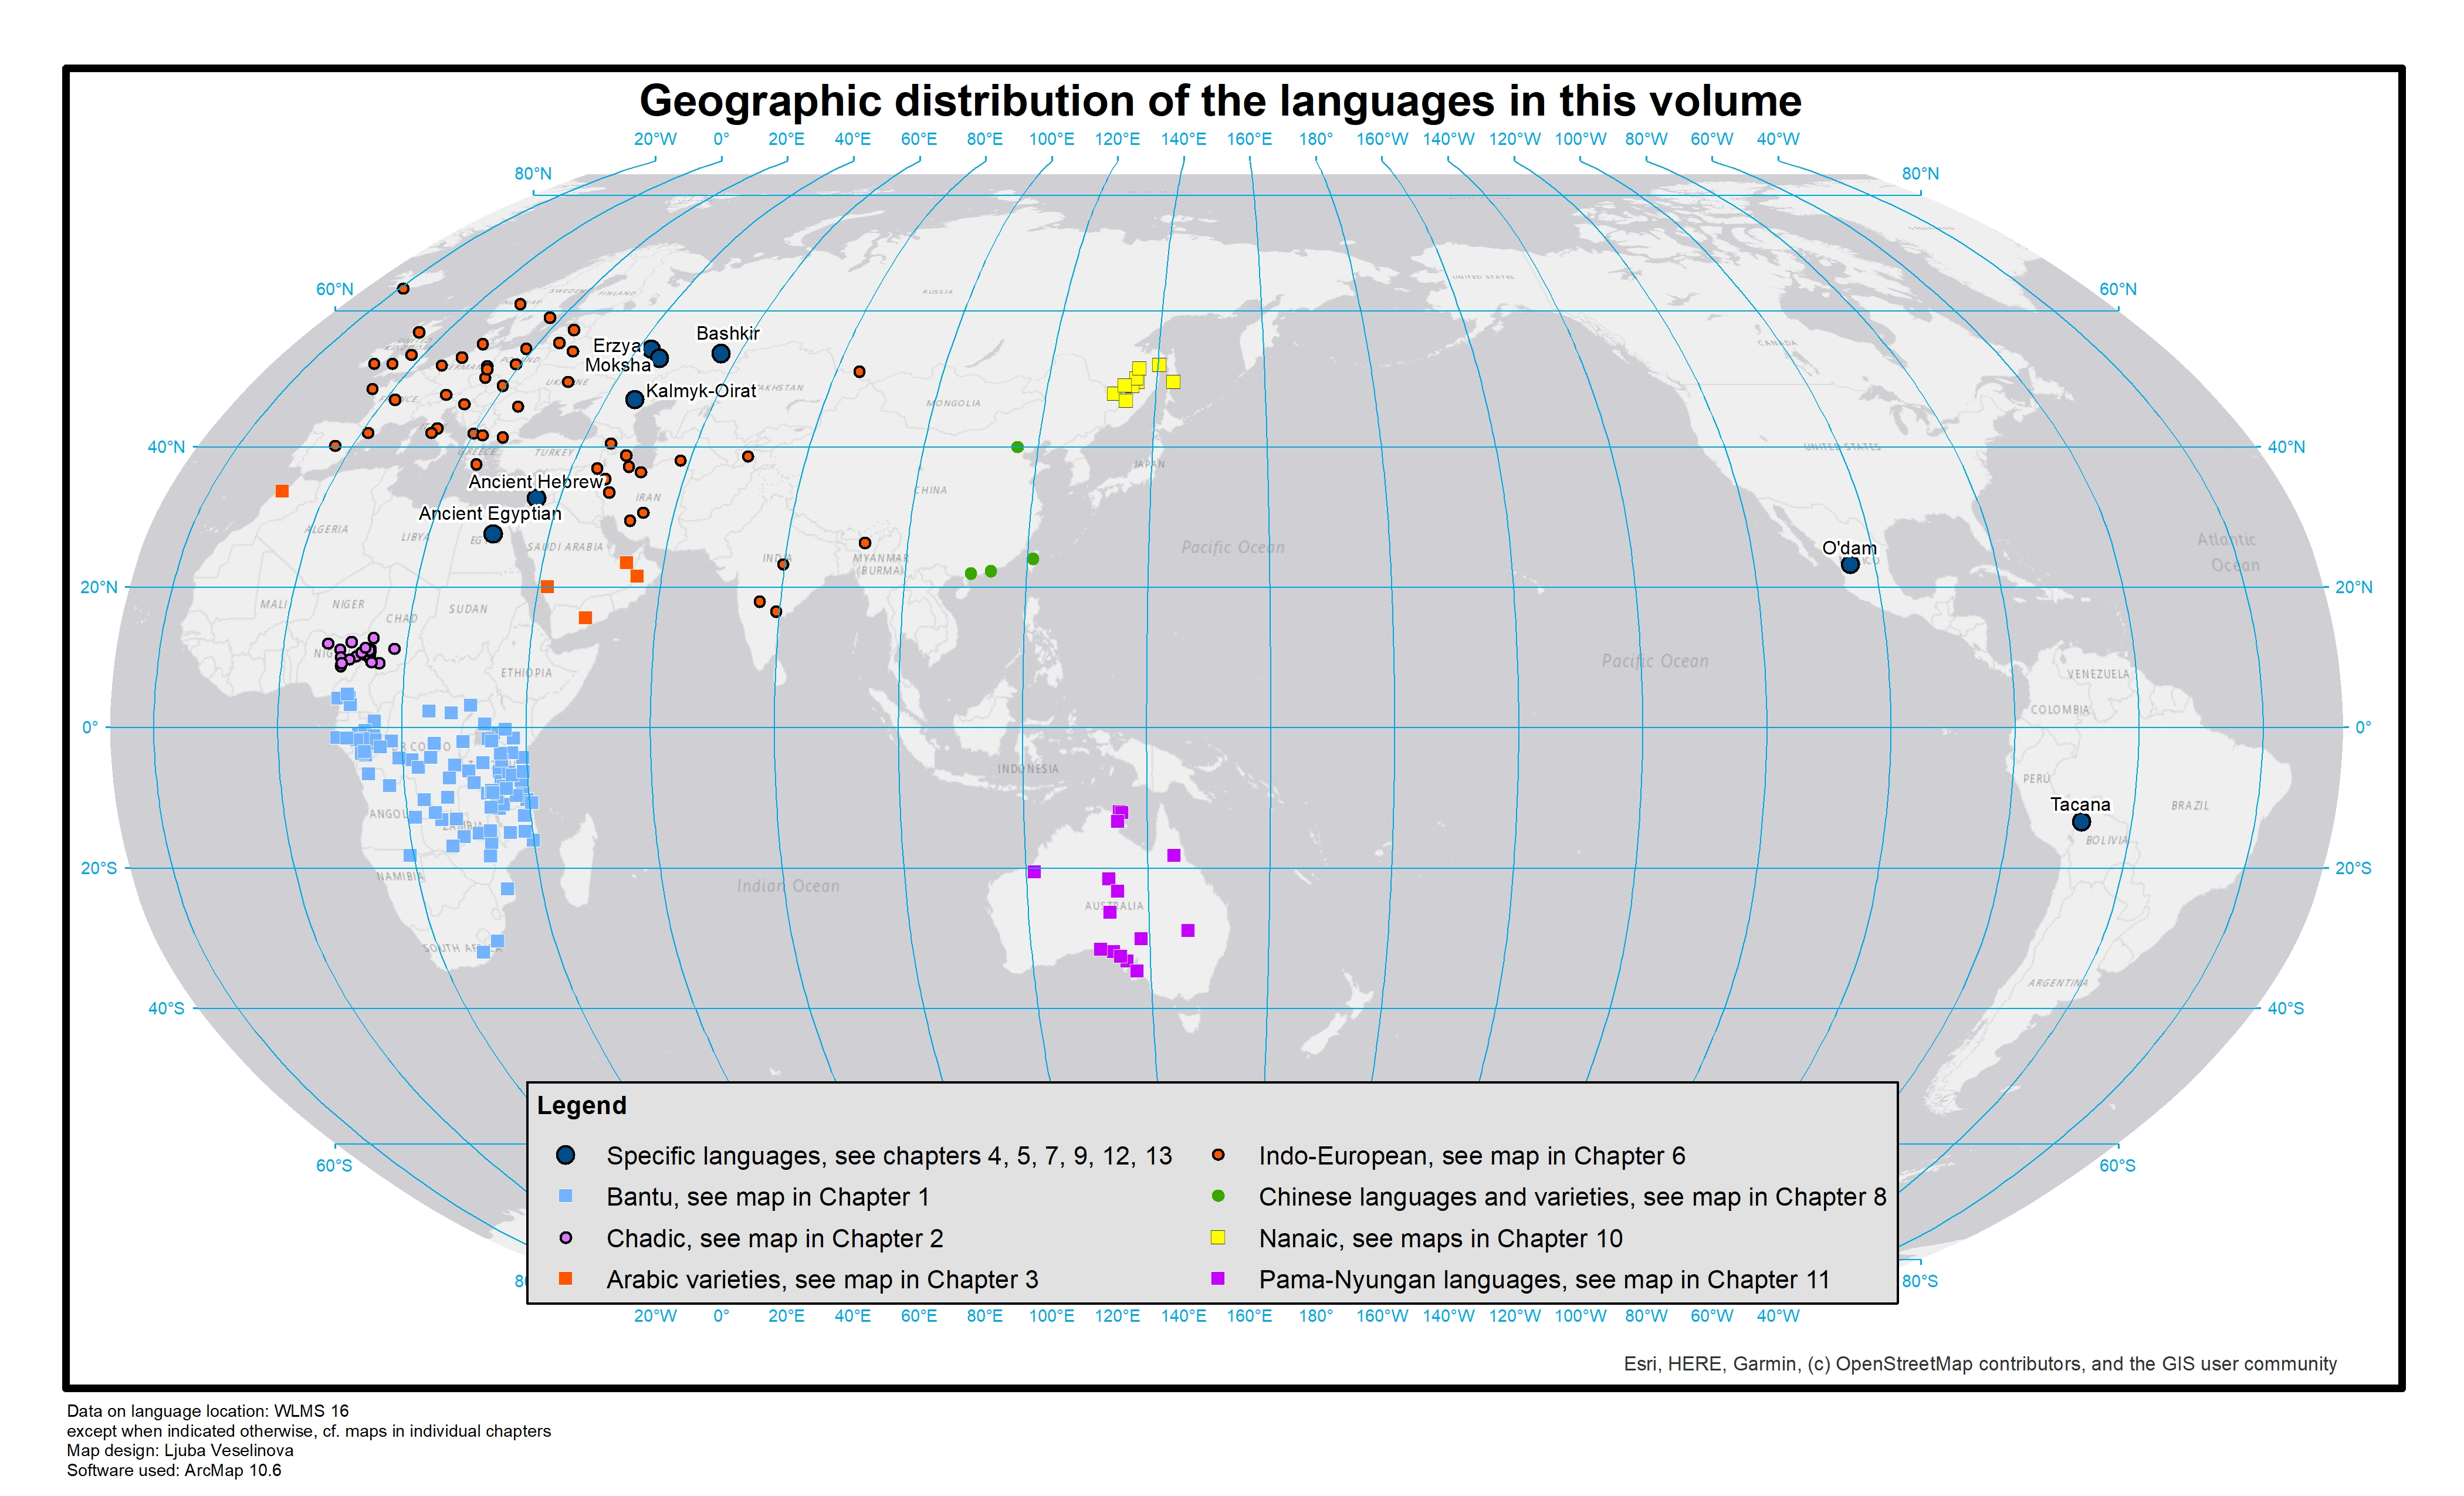
\includegraphics[width=\textwidth]{figures/All_langs_in_book.jpg}
    \caption{The languages and families analyzed in detail}
    \label{fig:all-langs-in-book}
\end{sidewaysfigure}


{\sloppy\printbibliography[heading=subbibliography,notkeyword=this]}
\end{document}
